\documentclass[11pt,a4paper]{article}

% ---------------------------------------------------------------------------
% PACKAGES
% ---------------------------------------------------------------------------
\usepackage[utf8]{inputenc}
\usepackage[T1]{fontenc}
\usepackage[margin=1in]{geometry}
\usepackage{amsmath,amssymb,amsthm}
\usepackage{mathtools}
\usepackage{graphicx}
\usepackage{tikz}
\usetikzlibrary{positioning,arrows.meta,calc,shapes.geometric}
\usepackage{enumitem}
\usepackage{booktabs}
\usepackage{longtable}
\usepackage{array}
\usepackage{colortbl}
\usepackage{xcolor}
\usepackage{listings}
\usepackage{fancyhdr}
\usepackage{hyperref}
\usepackage{titlesec}
\usepackage{mdframed}
\usepackage{tcolorbox}
\usepackage{float}
\usepackage{caption}
\usepackage{verbatim}
\usepackage{multirow}

% ---------------------------------------------------------------------------
% COLOURS
% ---------------------------------------------------------------------------
\definecolor{primary}{RGB}{25,42,86}
\definecolor{secondary}{RGB}{52,152,219}
\definecolor{accent}{RGB}{231,76,60}
\definecolor{success}{RGB}{22,160,133}
\definecolor{codebg}{RGB}{244,246,248}
\definecolor{notebg}{RGB}{255,249,229}
\definecolor{warnbg}{RGB}{255,235,230}
\definecolor{tipbg}{RGB}{230,248,238}
\definecolor{linkcol}{RGB}{41,128,185}
\definecolor{thinkbg}{RGB}{239,239,255}
\definecolor{storybg}{RGB}{242,244,234}
\definecolor{softpurple}{RGB}{142,68,173}
\definecolor{warmgray}{RGB}{120,120,120}

% ---------------------------------------------------------------------------
% HYPERREF
% ---------------------------------------------------------------------------
\hypersetup{
  colorlinks=true,
  linkcolor=linkcol,
  urlcolor=linkcol,
  citecolor=linkcol,
  pdftitle={Learning Cybersecurity AI from ZERO - A Friendly Tutorial},
  pdfauthor={SIH-26153 Team}
}

% ---------------------------------------------------------------------------
% HEADER / FOOTER
% ---------------------------------------------------------------------------
\pagestyle{fancy}
\fancyhf{}
\fancyhead[L]{\small\textcolor{primary}{\textbf{From ZERO to Hero\ |\ Cybersecurity AI}}}
\fancyhead[R]{\small\textcolor{secondary}{\thepage}}
\renewcommand{\headrulewidth}{0.5pt}
\renewcommand{\headrule}{\color{secondary}\hrule width\headwidth height 0.5pt}

% ---------------------------------------------------------------------------
% SECTION FORMATTING
% ---------------------------------------------------------------------------
\titleformat{\section}
  {\Large\bfseries\color{primary}}{\thesection.}{0.6em}{}
  [{\color{secondary}\titlerule[1pt]}]
\titleformat{\subsection}
  {\large\bfseries\color{secondary}}{\thesubsection}{0.6em}{}
\titleformat{\subsubsection}
  {\normalsize\bfseries\color{primary}}{\thesubsubsection}{0.6em}{}

% ---------------------------------------------------------------------------
% CUSTOM BOXES
% ---------------------------------------------------------------------------
\newtcolorbox{keybox}{
  colback=notebg,
  colframe=secondary,
  boxrule=0.8pt,
  title={\color{primary}\textbf{Key Idea --- Remember This!}},
  fonttitle=\bfseries,
  coltitle=black,
  left=6pt,right=6pt,top=4pt,bottom=4pt
}

\newtcolorbox{warnbox}{
  colback=warnbg,
  colframe=accent,
  boxrule=0.8pt,
  title={\color{primary}\textbf{Common Mistake --- Don't Do This!}},
  fonttitle=\bfseries,
  coltitle=black,
  left=6pt,right=6pt,top=4pt,bottom=4pt
}

\newtcolorbox{tipbox}{
  colback=tipbg,
  colframe=success,
  boxrule=0.8pt,
  title={\color{primary}\textbf{Teacher's Tip --- For Your Project}},
  fonttitle=\bfseries,
  coltitle=black,
  left=6pt,right=6pt,top=4pt,bottom=4pt
}

\newtcolorbox{examplebox}{
  colback=white,
  colframe=primary,
  boxrule=0.8pt,
  title={\color{primary}\textbf{Let's Work Through an Example Together}},
  fonttitle=\bfseries,
  coltitle=black,
  left=6pt,right=6pt,top=4pt,bottom=4pt
}

\newtcolorbox{storybox}{
  colback=storybg,
  colframe=success,
  boxrule=0.8pt,
  title={\color{primary}\textbf{Story Time --- An Analogy to Remember}},
  fonttitle=\bfseries,
  coltitle=black,
  left=6pt,right=6pt,top=4pt,bottom=4pt
}

\newtcolorbox{yourturn}{
  colback=thinkbg,
  colframe=accent!70,
  boxrule=0.8pt,
  title={\color{primary}\textbf{Your Turn! --- Try It Yourself (No Pressure)}},
  fonttitle=\bfseries,
  coltitle=black,
  left=6pt,right=6pt,top=4pt,bottom=4pt
}

\newtcolorbox{recap}{
  colback=tipbg,
  colframe=success!60,
  boxrule=0.8pt,
  title={\color{primary}\textbf{Quick Recap --- What We Just Learned}},
  fonttitle=\bfseries,
  coltitle=black,
  left=6pt,right=6pt,top=4pt,bottom=4pt
}

\newtcolorbox{imaginebox}{
  colback=thinkbg,
  colframe=softpurple!70,
  boxrule=0.8pt,
  title={\color{primary}\textbf{Imagine This --- Picture It in Your Mind}},
  fonttitle=\bfseries,
  coltitle=black,
  left=6pt,right=6pt,top=4pt,bottom=4pt
}

\newtcolorbox{jargonbox}{
  colback=notebg,
  colframe=warmgray,
  boxrule=0.8pt,
  title={\color{primary}\textbf{Word Bank --- New Word Alert!}},
  fonttitle=\bfseries,
  coltitle=black,
  left=6pt,right=6pt,top=4pt,bottom=4pt
}

% ---------------------------------------------------------------------------
% CODE STYLE
% ---------------------------------------------------------------------------
\lstdefinestyle{pystyle}{
  language=Python,
  basicstyle=\ttfamily\small,
  keywordstyle=\color{primary}\bfseries,
  commentstyle=\color{success}\itshape,
  stringstyle=\color{accent},
  backgroundcolor=\color{codebg},
  frame=single,
  rulecolor=\color{secondary!50},
  breaklines=true,
  showstringspaces=false,
  numbers=left,
  numberstyle=\tiny\color{gray},
  numbersep=8pt,
  tabsize=4
}
\lstset{style=pystyle}

% ---------------------------------------------------------------------------
% DOCUMENT
% ---------------------------------------------------------------------------
\begin{document}

% ===========================================================================
% TITLE PAGE
% ===========================================================================
\begin{titlepage}
\centering
\vspace*{0.6cm}
{\color{accent}\rule{\textwidth}{2pt}}\\[0.5cm]
{\Huge\bfseries\color{primary}
From ZERO to Hero}\\[0.3cm]
{\LARGE\bfseries\color{primary}
in Cybersecurity AI}\\[0.45cm]
{\Large\textcolor{secondary}{A Super-Friendly Tutorial for Absolute Beginners}}\\[0.35cm]
{\large\textcolor{warmgray}{\textit{No Prior Knowledge Needed. We Start From Scratch.}}}\\[0.35cm]
{\color{accent}\rule{\textwidth}{2pt}}\\[0.9cm]

{\Large\textbf{Challenge:} SIH-26153}\\[0.25cm]
{\large\textit{AI-based Network Attack Forecasting from Network Traffic Data}}\\[0.9cm]

\begin{minipage}{0.84\textwidth}
\centering
\small
\emph{``Dear reader, if you have never written a line of code, never heard of
an IP address, and think AI is magic --- this book is for you. By the last
page, you will understand how to build an AI that can \textbf{dream about the
future of a computer network} and warn us before a hacker strikes. I will hold
your hand the whole way. Let's begin together.''}
\\[0.4cm]
--- \emph{Your Teacher}
\end{minipage}

\vfill
{\large\color{primary}\textbf{What We Will Learn Together}}\\[0.4cm]
{\small
\begin{tabular}{@{}c@{}}
\hline
Chapter 0:\quad The Absolute Basics (What Even Is a Network? What Is AI?) \\
Chapter 1:\quad How Messages Travel on the Internet (Network Telemetry) \\
Chapter 2:\quad How Hackers Attack Step-by-Step (Lifecycles \& Datasets) \\
Chapter 3:\quad Teaching AI to Imagine the Future (World Models) \\
Chapter 4:\quad Making AI Explain Its Decisions (Interpretability) \\
Chapter 5:\quad Turning Your AI Into a Real Product (Systems) \\
\hline
\end{tabular}}
\vfill
{\small\textit{Generated with \LaTeX\ \textbullet\ SIH-26153 Tutorial Notes}}
\end{titlepage}

% ---------------------------------------------------------------------------
% TABLE OF CONTENTS
% ---------------------------------------------------------------------------
\newpage
\tableofcontents
\newpage

% ===========================================================================
% HOW TO USE THIS BOOK
% ===========================================================================
\section*{How to Use This Book (Please Read This First!)}
\addcontentsline{toc}{section}{How to Use This Book}
\markboth{How to Use This Book}{}

Hello! Before we learn anything, let me tell you \textbf{how} to read this book
so you don't get confused or scared.

\medskip
\noindent\textbf{1. Every hard word is explained the FIRST time it appears.}
When you see a box that says \textbf{Word Bank}, that is me stopping to say:
``Hey, this is a new word --- here is what it means in simple English.'' You
never need to Google anything while reading.

\medskip
\noindent\textbf{2. Every idea starts with a story or a picture.}
Your brain loves stories. So before I show you a scary formula, I will say
``Imagine you are mailing a letter...'' Once you get the picture, the formula
will feel friendly, not scary.

\medskip
\noindent\textbf{3. Boxes have meanings. Learn them once:}
\begin{itemize}[leftmargin=1.6em,itemsep=2pt]
  \item \textbf{Word Bank} --- a new term, explained like you are 10 years old.
  \item \textbf{Imagine This} --- close your eyes and picture an everyday scene.
  \item \textbf{Story Time} --- a little tale to make the idea stick in memory.
  \item \textbf{Key Idea} --- the one thing you MUST remember from this section.
  \item \textbf{Let's Work Through an Example} --- we solve something together,
        step by step, with numbers.
  \item \textbf{Your Turn} --- a tiny exercise for you. No grading! Just to
        check you got it. Try with pen and paper.
  \item \textbf{Quick Recap} --- a 3-line summary before we move on.
  \item \textbf{Common Mistake} --- the trap every beginner falls into.
  \item \textbf{Teacher's Tip} --- how this connects to your actual project.
\end{itemize}

\medskip
\noindent\textbf{4. You do NOT need to be good at maths.}
Where maths appears, I will tell you what every symbol means in plain words,
and what the equation is \emph{trying to say}. You can understand the story
without memorising the maths.

\medskip
\noindent\textbf{5. Read with a pencil.}
Underline, scribble ``aha!'' in the margins, draw little hearts. Active reading
beats passive reading every time.

\medskip
If you are ready, turn the page. Chapter 0 is waiting --- and it assumes you
know \emph{literally nothing}. Perfect place to start.

\newpage

% ===========================================================================
% CHAPTER 0 - ABSOLUTE BASICS
% ===========================================================================
\section{Chapter 0: The Absolute Basics \\
\small What Even Is a Network? What Is AI? Let's Start From Zero.}
\label{sec:zero}

This chapter is for the true beginner. If you already know what an IP address
and machine learning are, you can skim it. If not, welcome --- we are going to
build your foundation block by block, with zero shame and lots of pictures in
your mind.

\subsection{0.1 What Is a Computer Network? Roads and Houses.}

\begin{imaginebox}
Close your eyes and picture your town. There are \textbf{houses} (computers,
phones, servers). There are \textbf{roads} (wires and Wi-Fi) connecting them.
There are \textbf{letters and parcels} (messages) travelling on those roads
from one house to another. That whole town --- houses plus roads plus the
system for sending letters --- is a \textbf{computer network}.

The \textbf{Internet} is just a \emph{really big} town where the houses are all
over the world and the roads are a mix of cables under the ocean and radio
waves through the air.
\end{imaginebox}

That is it. When we say ``network traffic,'' we just mean ``all the letters
travelling on all the roads at a given time.'' When we say ``network
security,'' we mean ``making sure bad letters don't cause harm, and that no
one sneaks into a house they shouldn't.''

\begin{jargonbox}
\textbf{Network} = a group of connected computers that can send messages to
each other.\\
\textbf{Internet} = the biggest network in the world, connecting billions of
devices.\\
\textbf{Traffic} = all the messages moving around the network right now.\\
\textbf{Device / Host} = one house in the town (your laptop, a server, a phone).
\end{jargonbox}

\subsection{0.2 What Is Data? Letters, Forms, and Report Cards.}

\textbf{Data} just means ``information written down so a computer can read it.''

Think of three levels:
\begin{itemize}[leftmargin=1.6em,itemsep=2pt]
  \item \textbf{Raw data} = the actual letter inside the envelope. The words
        ``Hi, please send me the file cats.jpg''.
  \item \textbf{Features} = a \emph{summary} someone made from the raw data so
        it is easier to compare. Like a report card: instead of reading every
        homework page, you see ``Maths: 85, Science: 90.''
  \item \textbf{Label} = the answer written by a teacher: ``This letter is
        \textbf{safe}'' or ``This letter is \textbf{dangerous}''.
\end{itemize}

\begin{keybox}
\textbf{Features} are the clues we give to the AI.\\
\textbf{Labels} are the correct answers we use to teach the AI.\\
A \textbf{dataset} is a big collection of clues + answers, like a big folder
of past exam papers with answer keys.
\end{keybox}

\subsection{0.3 What Is Cybersecurity? Guards, Burglars, and Alarms.}

\begin{storybox}
Imagine a museum. It has many rooms (computers), doors (ports --- we will learn
this!), and guards (security software). A burglar wants to steal a painting
(data). They might: look through windows first (scan), try a back door
(break in), sneak from room to room (lateral movement), call a friend outside
for instructions (command and control), and finally carry the painting out
(exfiltration).

\textbf{Cybersecurity} is the job of stopping that burglar --- not after the
painting is gone, but \emph{as early as possible}, ideally while they are
still looking through the windows.
\end{storybox}

Old security worked like a photo album: ``If you see THIS exact face, it's a
burglar.'' But burglars change faces. Modern AI security is like learning the
\emph{behaviour} of burglars --- the \emph{pattern} of how they move --- so
you can spot even a new burglar you have never seen before.

\subsection{0.4 What Is Artificial Intelligence and Machine Learning? Teaching a Child.}

\begin{jargonbox}
\textbf{Artificial Intelligence (AI)} = making computers do things that normally
need human intelligence (recognising, deciding, predicting).\\[2pt]
\textbf{Machine Learning (ML)} = a way to do AI where we don't write fixed
rules, but instead \emph{show the computer many examples} and let it \emph{learn
the pattern} itself. Like teaching a child to recognise cats by showing 1000
cat photos, not by writing ``cats have pointy ears.''
\end{jargonbox}

How does ML work? In super simple terms:

\begin{enumerate}[leftmargin=1.8em,itemsep=2pt]
  \item You collect a \textbf{dataset}: many examples (features) with correct
        answers (labels).
  \item You choose a \textbf{model}: a maths recipe with knobs you can turn.
        At first the knobs are random, so the model's guesses are terrible.
  \item You \textbf{train}: show the model one example, let it guess, tell it
        ``you were wrong by this much,'' and it turns its knobs a tiny bit to
        be less wrong. Do this millions of times.
  \item You \textbf{test}: show it \emph{new} examples it has never seen and
        see if it still guesses well. If yes, it \emph{learned}, not memorised.
  \item You \textbf{deploy}: use it in the real world to make predictions.
\end{enumerate}

\begin{imaginebox}
Think of baking. Your first cake is awful. You taste it, note ``too much
salt,'' adjust the recipe, bake again. After 100 cakes, you are a good baker.
The ``tasting and adjusting'' is training. The ``try a new recipe on a friend''
is testing. That is literally all machine learning is.
\end{imaginebox}

\subsection{0.5 What Is a Feature Vector? Ingredients List.}

A \textbf{vector} is just a \emph{list of numbers in a fixed order}. A
\textbf{feature vector} is the list of clues for one example.

Example: one network conversation (one ``flow'') might become:
\[
[\; 80,\;  421,\;  0.04,\;  3,\;  0.98\;]
\]
In our code this means: destination port 80, 421 bytes, duration 0.04 seconds,
3 packets, and some timing score 0.98. The \emph{order} matters --- position 1
is always the port, position 2 always the bytes, etc. The AI reads this list
like you read ingredients: flour, sugar, eggs \dots

\subsection{0.6 What Do Probability, $P$, and Those Maths Symbols Mean?}

You will see things like $P(A \mid B)$. Do not panic. Here is the decoder ring:

\begin{itemize}[leftmargin=1.6em,itemsep=2pt]
  \item \textbf{$P(X)$} means ``the probability (chance) that $X$ happens.''
        $P=0$ means never, $P=1$ means always, $P=0.8$ means 80\% chance.
  \item \textbf{$P(A \mid B)$} means ``the probability of $A$ \emph{given that}
        $B$ happened.'' Like ``chance of rain GIVEN that clouds are dark.''
  \item \textbf{$S_t$} means ``the state of the network at time $t$'' (snapshot
        at minute $t$). $S_{t+1}$ is the next minute.
  \item \textbf{$\sigma(x)$} (sigmoid) = a squishy function that takes any
        number and squishes it to between 0 and 1, like a probability.
  \item \textbf{$\tanh(x)$} = similar, but squishes to between $-1$ and $1$.
  \item \textbf{$\odot$} = multiply each item in one list with the matching
        item in another list (element-by-element).
  \item \textbf{$W$ and $b$} = knobs the AI turns during training (weights and
        biases). $W$ is like ``how strongly to listen to each clue,'' $b$ is
        ``a small nudge.''
\end{itemize}

You don't need to calculate these by hand. Just know the \emph{story} each
equation tells: ``combine the old memory with the new clues, decide what to
keep, what to forget, and what to output.''

\begin{recap}
\textbf{You now know:} networks are towns with roads; traffic is letters on
roads; data = written-down information; features = summaries; labels = answers;
AI learns by tasting and adjusting like a baker; a feature vector is an
ingredients list; $P$ means chance. You are ready for Chapter 1!
\end{recap}

\newpage

% ===========================================================================
% CHAPTER 1
% ===========================================================================
\section{Chapter 1: How Messages Travel on the Internet \\
\small Network Telemetry \& Feature Engineering}

\emph{Telemetry} sounds scary. It just means ``measuring from far away.'' A
weather station that radios temperature to your phone is telemetry. Here,
\emph{network telemetry} means ``measuring what is happening on the network
and sending those measurements to our AI.''

\subsection{1.1 The Big Picture: The Postal System of the Internet}
\label{sec:tcpip}

\begin{imaginebox}
You want to send a birthday gift to your friend. What do you do?

You put the gift (the \textbf{actual message}, like ``Please show me
cats.jpg'') inside a \textbf{small box} and write ``Deliver to Room 80,
Handle with care''. That small box goes inside a \textbf{bigger box} with
``From: House 1.2.3.4, To: House 5.6.7.8''. That bigger box goes inside an
even bigger \textbf{mail truck envelope} for the road.

At your friend's house, they unwrap layer by layer: truck envelope off,
then big box, then small box, until the gift appears.

The Internet does EXACTLY this. We call it \textbf{encapsulation}: each layer
wraps the layer above. And \textbf{decapsulation} is unwrapping at the other
end.
\end{imaginebox}

We name those layers like floors of a building:

\begin{center}
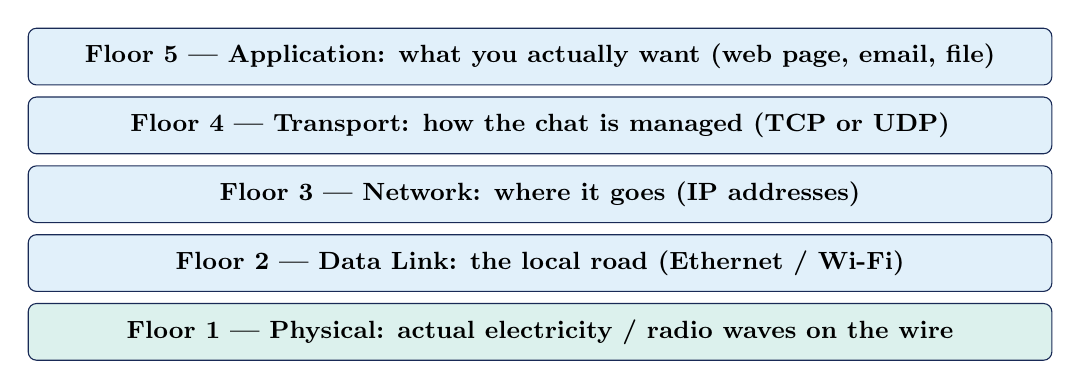
\begin{tikzpicture}[
  layer/.style={draw=primary, fill=secondary!15, rounded corners=3pt,
    minimum width=13cm, minimum height=0.72cm, font=\bfseries\small}
]
\node[layer] (L5) {Floor 5 --- Application: what you actually want (web page, email, file)};
\node[layer, below=0.14cm of L5] (L4) {Floor 4 --- Transport: how the chat is managed (TCP or UDP)};
\node[layer, below=0.14cm of L4] (L3) {Floor 3 --- Network: where it goes (IP addresses)};
\node[layer, below=0.14cm of L3] (L2) {Floor 2 --- Data Link: the local road (Ethernet / Wi-Fi)};
\node[layer, below=0.14cm of L2, fill=success!15] (L1) {Floor 1 --- Physical: actual electricity / radio waves on the wire};
\end{tikzpicture}
\end{center}
\noindent\emph{Each floor adds its own label (header). The Transport letter goes
inside the Network parcel which goes inside the Data-Link truck.}

\begin{keybox}
For catching hackers, you will spend 95\% of your time on just \textbf{two
floors}:
\begin{itemize}[leftmargin=1.6em,itemsep=1pt]
  \item \textbf{Network (IP)} = the house addresses (who sent, who receives).
  \item \textbf{Transport (TCP/UDP)} = the apartment numbers and chat rules
        (which door, and is the conversation polite and reliable?).
\end{itemize}
Everything called a ``packet'' or ``flow'' lives in these headers.
\end{keybox}

\subsection{1.2 IP Addresses and Ports: House Numbers and Apartment Doors}
\label{sec:addresses}

This confuses everyone at first. Let's make it crystal clear.

\begin{jargonbox}
\textbf{IP address} = the street address of a house (computer) on the Internet.

Example: \texttt{192.168.1.10} or \texttt{142.250.182.14} (Google). Two houses
can't have the same address if they want to receive mail.

\textbf{Port} = the apartment/door number \emph{inside} a house. One house can
have many doors for different services.

Common doors: 80 = web, 443 = secure web, 22 = secure login (SSH), 53 = address
book lookup (DNS).

\textbf{Protocol number} = which language the letter inside is written in:
6 = TCP (reliable chat), 17 = UDP (quick postcard), 1 = ICMP (ping / ``are you
there?'').
\end{jargonbox}

So when you see \texttt{192.168.1.10:52184 -> 142.250.182.14:443 with TCP}, read
it as: ``From house 192.168.1.10, door 52184, to Google's house at door 443
(secure web), speaking TCP.''

\begin{yourturn}
Your computer right now has an IP address. On Windows type \texttt{ipconfig},
on Mac/Linux type \texttt{ifconfig} in the terminal. Can you find it? What
does it start with? Now open a browser and go to \texttt{google.com}. You just
sent packets to port 443. Magic!
\end{yourturn}

\subsection{1.3 The IP Header: Writing on the Outside of the Envelope}
\label{sec:ipheader}

Every letter (IP packet) has writing on the outside called a \textbf{header}.
It is usually 20 bytes long (tiny!). Here is what is written there, in plain
English:

\begin{itemize}[leftmargin=1.6em,itemsep=2pt]
  \item \textbf{Source IP} --- who sent it. (``From:'')
  \item \textbf{Destination IP} --- who gets it. (``To:'')
  \item \textbf{Time To Live (TTL)} --- a countdown number, like ``this letter
        may pass through at most 64 post offices. Each office subtracts 1. If it
        hits 0, throw it away.'' Weird TTL jumps hint at \textbf{spoofing}
        (someone faking the From address) or a strangely long route.
  \item \textbf{Protocol} --- which inner language (6 = TCP, 17 = UDP).
  \item \textbf{Flags + Fragment info} --- ``is this letter torn into pieces?''
        Big letters sometimes get torn into \textbf{fragments} to fit through a
        small mail slot. Clever hackers tear their bad letters into tiny pieces
        so no single piece looks bad. This is an \textbf{evasion trick}.
  \item \textbf{Total Length} --- how big the whole thing is, in bytes.
\end{itemize}

\begin{storybox}
\textbf{Fragment trick --- the scattered puzzle:}
A burglar wants to smuggle a long message past a guard who checks every letter.
So they tear the message into one word per letter and mail them separately.
No single letter looks suspicious. But together, they form the plan. That is
why we need \textbf{packet-level} clues, not just summaries --- to catch the
scattered puzzle.
\end{storybox}

\subsection{1.4 The TCP Header: The Rules of a Polite Phone Call}
\label{sec:tcpheader}

TCP is the \textbf{polite, reliable} way to talk. If IP is the envelope, TCP
is the \emph{conversation style} inside. It promises: ``Your words will arrive,
in order, without mistakes. If not, I will resend.''

It does this with a small header that rides inside the IP envelope:

\begin{itemize}[leftmargin=1.6em,itemsep=2pt]
  \item \textbf{Source Port / Destination Port} --- which doors (see above).
  \item \textbf{Sequence Number \& Acknowledgment Number} --- page numbers for
        your chat. ``I sent pages 1-10, did you get them?'' ``Got 1-10, send
        11 onwards.''
  \item \textbf{Flags} --- tiny single-word instructions. These are GOLD for
        catching hackers. Let's learn them like verbs:
        \begin{itemize}[leftmargin=2.2em,itemsep=1pt]
          \item \textbf{SYN} = ``Hello, can we talk?'' (synchronize)
          \item \textbf{ACK} = ``Got it!'' (acknowledge)
          \item \textbf{FIN} = ``Goodbye, I'm done.'' (finish)
          \item \textbf{RST} = ``Go away, stop talking!'' (reset / abort)
          \item \textbf{PSH} = ``Deliver this NOW, don't wait.'' (push)
          \item \textbf{URG} = ``This is urgent!'' (urgent)
        \end{itemize}
  \item \textbf{Window Size} --- ``I can accept this many more words before my
        desk is full.'' Weird window sizes are a fingerprint of
        \emph{port scanners} and hacking tools.
\end{itemize}

\begin{examplebox}
\textbf{The TCP Handshake --- two people meeting for the first time:}

\begin{enumerate}[label=\textbf{\arabic*.},leftmargin=1.8em,itemsep=2pt]
  \item You: ``Hi, can we talk?'' (\textbf{SYN})
  \item Them: ``Sure, and can \emph{I} also talk to you? Got your hello.'' (\textbf{SYN + ACK})
  \item You: ``Great, got your reply, let's chat!'' (\textbf{ACK})
\end{enumerate}

Every normal chat starts exactly like this. Three messages. Always.

Now: a \textbf{port scanner} is like a burglar who knocks on \emph{every door}
of a building (port 1, port 2, port 3 \dots\ up to 65535) going
``Hello? Hello? Hello?'' but \emph{never waits for the full hello back}.
They just send tons of SYN and vanish. That pattern --- \emph{many SYNs, very
few ACKs} --- is super easy for our AI to spot. That is a \textbf{feature} we
will use.
\end{examplebox}

\subsection{1.5 UDP: The Postcard (Quick but No Guarantee)}
\label{sec:udp}

UDP is TCP's laid-back cousin. It just throws a postcard and hopes it arrives.
No hello, no confirmation, no resending. It has only four things: from-port,
to-port, length, and a tiny check.

It is perfect for things where speed beats perfection: looking up an address
(DNS), voice calls, video. But because it doesn't say hello, it is easy to
\textbf{fake}. Attackers love sending fake postcards pretending to be someone
else (``DNS amplification'' attacks). Postcards are hard to trace.

\begin{recap}
\textbf{So far:} Internet = postal system with layers. IP = house address.
Port = door number. TCP = polite phone call with SYN/ACK/FIN. UDP = postcard.
Flags are verbs that reveal hacker behaviour.
\end{recap}

\subsection{1.6 From Many Letters to One Summary: What Is a Flow?}
\label{sec:flow}

\begin{imaginebox}
Imagine you are a teacher watching a playground. You could write down
\emph{every single word} every kid says --- that is \textbf{packet-level}.
Or you could write one summary per \emph{conversation}: ``Asha and Ben talked
for 2 minutes, exchanged 5 messages, Asha spoke 3 times.'' That summary is a
\textbf{flow}.

Flows are summaries. They are MUCH smaller and they already tell you the
story.
\end{imaginebox}

\begin{keybox}
A \textbf{flow} = one summary line for all packets that share the same
\textbf{5-tuple} (the ID card of a conversation):
\[
( \texttt{who-sent-IP},\; \texttt{who-sent-port},\; \texttt{who-got-IP},\; \texttt{who-got-port},\; \texttt{protocol} )
\]
We usually combine both directions (you-to-me and me-to-you) into one
\textbf{bidirectional flow} so the summary is complete.
\end{keybox}

What does one flow record contain? Think of it like a report card for that
conversation:

\begin{table}[H]
\centering
\caption{A Flow Record Is a Report Card for One Conversation}
\small
\begin{tabular}{@{}ll@{}}
\toprule
\emph{Group} & \emph{What it tells you (in plain words)} \\
\midrule
Who & From which house/door to which house/door, which language (TCP/UDP) \\
When & When it started, when it ended, how long it lasted \\
How much & How many bytes and packets each side sent \\
How fast & Bytes per second, packets per second (throughput) \\
Rhythm & Time \emph{between} packets: fastest gap, slowest gap, average gap \\
Size & Smallest packet, biggest packet, average packet size \\
Verbs & How many SYN, ACK, PSH, RST flags were seen \\
Pauses & How long the chat was active vs.\ idle \\
\bottomrule
\end{tabular}
\end{table}

These numbers are the \textbf{features} your AI will learn from. Instead of
reading every word, the AI reads the report card --- and that is enough to
tell normal chats from hacker chats, most of the time.

\subsection{1.7 NetFlow and IPFIX: The Standard Way to Write Report Cards}
\label{sec:ipfix}

Routers (the post offices) don't keep every letter. They write \emph{report
cards} (flows) and send them to a collector. The language for writing those
report cards has two versions:

\begin{itemize}[leftmargin=1.6em,itemsep=2pt]
  \item \textbf{NetFlow} (made by Cisco) = the original report-card format.
        Fixed fields, like a printed form.
  \item \textbf{IPFIX} (the newer, official standard) = a \emph{customisable}
        form. You can add any field you want via \textbf{templates}: ``also
        include TCP flags, also include app name.'' For security this is
        wonderful --- we can ask the post office to include exactly the clues
        we need.
\end{itemize}

For your project, just remember: NetFlow/IPFIX = the system that \emph{creates
and exports} flow summaries. When you load a CSV with 80 columns, you are
reading exported flows.

\subsection{1.8 Two Levels Are Better Than One: Flows AND Packets}
\label{sec:levels}

\begin{itemize}[leftmargin=1.6em,itemsep=2pt]
  \item \textbf{Flow-level clues} (the report card) catch \emph{loud} attacks:
        floods (too many packets), exfiltration (too many bytes out).
  \item \textbf{Packet-level clues} (reading actual envelopes) catch
        \emph{sneaky} attacks: weird TTL, tiny fragments, strange window sizes
        that look normal in the report card but are odd up close.
\end{itemize}

Your challenge says: use \textbf{both} levels. Two eyes see more than one.
A flow that looks normal might still have packet-level oddities that give the
hacker away.

\begin{recap}
\textbf{Chapter 1 recap:} Networks are postal towns. IP = house, port = door,
TCP = polite call with verbs (SYN/ACK/FIN/RST), UDP = postcard. A \textbf{flow}
is a report card summarising one conversation (5-tuple). NetFlow/IPFIX exports
those report cards. Use flow-level for loud attacks, packet-level for sneaky
ones.
\end{recap}

\subsection{1.9 Hands On: Reading Packets with Python (Line by Line)}
\label{sec:parsing}

You might be thinking: ``Do I need to be a coder?'' For this project, a little
Python is enough, and I will explain every line like you have never coded before.

\begin{jargonbox}
\textbf{Python} = a human-friendly programming language. Like giving written
instructions to a very obedient robot.\\[2pt]
\textbf{Library} = a pre-written bundle of instructions someone else made so you
don't start from scratch. Like a recipe book.\\[2pt]
\textbf{PCAP file} = a file that contains saved network traffic --- a box of
saved letters you can open and study without being on the live network.\\
\textbf{Scapy} = a Python library that can open, read, and even create packets.
Pure Python, great for learning.\\
\textbf{PyShark} = another library that uses Wireshark (a famous network tool)
under the hood. Faster for huge files.
\end{jargonbox}

\begin{examplebox}
\textbf{Your first packet reader --- explained line by line:}
\begin{lstlisting}[language=Python]
from scapy.all import rdpcap, TCP, IP   # 1. Borrow tools from the Scapy recipe book

packets = rdpcap("traffic.pcap")        # 2. Open the saved box of letters. Now 'packets' is a list.

for pkt in packets[:5]:                 # 3. Look at just the first 5 letters, one by one.
    if IP in pkt and TCP in pkt:        # 4. Only care about letters that have BOTH an IP envelope AND a TCP letter inside.
        ip   = pkt[IP]                  # 5. Pull out the IP envelope to read it.
        tcp  = pkt[TCP]                 # 6. Pull out the TCP letter to read it.
        print(f"{ip.src}:{tcp.sport} -> {ip.dst}:{tcp.dport} "
              f"flags={tcp.flags} len={len(pkt)} ttl={ip.ttl}")
                                        # 7. Print: "From house:door -> To house:door  flags=...  size=...  ttl=..."
\end{lstlisting}

\textbf{What this does:} It opens a capture file, picks the first 5 TCP packets,
and prints who sent what to whom, with which flags, how big, and what TTL.
That is literally the raw material of your whole project.
\end{examplebox}

\begin{tipbox}
\textbf{Do you need to parse packets yourself?} If your dataset is already a
CSV of flows (like CIC-IDS, which we meet in Chapter 2), you can \emph{skip}
parsing and go straight to the next section. Only parse raw PCAPs when you
want packet-level detail or when your data is a PCAP. Parsing is the slowest
step --- always \textbf{save (cache)} your result so you don't re-parse every
time you run your code. Think of it as photocopying the letters once and
reusing the copies.
\end{tipbox}

\subsubsection{The Whole Pipeline in One Line}

\[
\texttt{PCAP file} \ \xrightarrow{\text{read each letter}} \ \text{rows of packets}
\ \xrightarrow{\text{group by 5-tuple}} \ \text{rows of flows}
\]
\[
\ \xrightarrow{\text{clean up numbers}} \ \text{feature table (matrix)}
\]

Each \emph{row} = one flow (one conversation). Each \emph{column} = one clue
(bytes, packets, flag counts \dots). This table is what the AI eats. Like a
spreadsheet where the AI reads every row.

\begin{yourturn}
If you have Python installed, try installing Scapy (\texttt{pip install scapy})
and running the code above on any small PCAP (you can download free ones from
\texttt{wireshark.org}). If you don't have a PCAP yet, that's fine --- just
read the code again and explain to a friend what line 4 does in your own words.
Teaching is the best way to learn.
\end{yourturn}

\subsection{1.10 Cutting Time into Slices: Windows and Discretisation}
\label{sec:windowing}

A single flow is one conversation. But a \textbf{hacker attack} is a
\emph{movie} with many scenes: first they look around, then they break in,
then they sneak around, then they steal. To see the movie, you must cut time
into \textbf{slices} (windows) and look at the whole picture inside each slice.

\begin{imaginebox}
Imagine a very long security camera recording. You can't watch it all at once.
So you cut it into 1-minute clips: Clip 1 (0:00--1:00), Clip 2 (1:00--2:00),
\dots\ For each clip you write a summary: ``2 people entered, 1 carried a bag
out.''

Those clips are \textbf{windows}. The summary of each clip is the
\textbf{state} your AI will see at that time step. The AI then watches the
\emph{sequence} of clips to learn the story.
\end{imaginebox}

\begin{keybox}
\textbf{Windowing} = cutting continuous time into \textbf{discrete (separate)
slices} so we can feed a \emph{sequence of snapshots} to the AI.

Without windows $\Rightarrow$ no sequence $\Rightarrow$ no story $\Rightarrow$
no World Model. Windows are how we turn time into something the AI can learn
from.
\end{keybox}

\subsubsection{How to Define a Window}

Pick a size $w$ (say, 60 seconds) and a slide $s$ (how far to move each time).

Window number $k$ covers time $[k \times s,\; k \times s + w)$. Two styles:

\begin{itemize}[leftmargin=1.6em,itemsep=2pt]
  \item \textbf{Tumbling windows}: $s = w$. Like cutting a cake with no overlap:
        [0--60), [60--120), [120--180) \dots\ No piece shares crumbs.
  \item \textbf{Sliding windows}: $s < w$. Like overlapping photos:
        [0--60), [30--90), [60--120) \dots\ More photos, smoother movie, but
        neighbouring photos look similar.
\end{itemize}

\begin{jargonbox}
\textbf{Discretisation} = turning smooth, continuous time (like ``3:17:04.392'')
into counted buckets (like ``the 3:17 bucket''). Once time is bucketed, we can
count things per bucket and the AI can handle it.
\end{jargonbox}

\subsubsection{Choosing How Big a Slice Should Be (Goldilocks)}

\begin{itemize}[leftmargin=1.6em,itemsep=2pt]
  \item \textbf{Too tiny} (e.g., 1 second) $\Rightarrow$ each slice has almost
        nothing, noisy, and you get a million slices. Hard to see the big
        picture.
  \item \textbf{Too huge} (e.g., 1 hour) $\Rightarrow$ a whole attack fits in
        one slice, so you can't see the stages. Blur.
  \item \textbf{Just right} = match the \emph{speed of what you want to catch}.
        A port scan is fast (seconds). Data theft is slower (minutes). Try a few
        sizes and see which works best on your data. In your project, try 30s or
        60s and compare.
\end{itemize}

\begin{warnbox}
\textbf{The Sneaky Cheating Trap with Windows:}

When you label your windows using the answer key (attack timeline), never cut
a \emph{single continuous attack} in half with one half in training and the
other half in testing. That lets the AI ``peek'' at the future. Always split
by \emph{time}: first 70\% of the movie for training, last 30\% for testing,
and keep whole attacks together. We will meet this again as ``data leakage''
in Chapter 2.
\end{warnbox}

\begin{recap}
\textbf{Chapter 1 recap in one paragraph:}
We cut the long movie of network traffic into window-slices, summarise each
slice (flows), and turn those summaries into a neat table of numbers. That
table is the AI's view of the world. Next, we learn what the \emph{bad
guys} actually do inside that movie.
\end{recap}

\newpage

% ===========================================================================
% CHAPTER 2
% ===========================================================================
\section{Chapter 2: How Hackers Attack Step-by-Step \\
\small Cybersecurity Attack Lifecycles \& Datasets}

\subsection{2.1 The Attacker's Playbook: MITRE ATT\&CK (The Big Map)}
\label{sec:mitre}

Before you can \emph{predict} a burglar, you must understand how burglars think.
Security experts around the world collected every trick real attackers have
ever used and wrote them into a giant, free, constantly updated playbook called
\textbf{MITRE ATT\&CK}. Think of it as the ``encyclopaedia of hacking steps.''

\begin{jargonbox}
\textbf{MITRE} = a non-profit research group in the USA that made the playbook.\\
\textbf{ATT\&CK} = stands for \textbf{A}dversarial \textbf{T}actics,
\textbf{T}echniques, and \textbf{C}ommon \textbf{K}nowledge.\\
\textbf{Tactic} = the \emph{WHY}: the attacker's goal at this stage. (``Why
are they doing this?'' --- e.g., ``to get inside.'')\\
\textbf{Technique} = the \emph{HOW}: the specific trick to achieve that goal.
(``How do they do it?'' --- e.g., ``by exploiting a bug in the website.'')\\
\textbf{Sub-technique} = an even more specific version of a technique.\\
\textbf{Procedure} = a real-world example of a hacker group using that technique.
\end{jargonbox}

Think of it like cooking:

\[
[\ \text{Tactics (the WHY --- the course)}\ ] \times
[\ \text{Techniques (the HOW --- the recipe)}\ ]
\]

Tactic = ``make dessert,'' Technique = ``bake a chocolate cake,'' Sub-technique
= ``use dark chocolate.''

\begin{storybox}
\textbf{The Burglar's Night --- The Same Steps, Every Time:}

A burglar rarely just runs in and grabs. They follow a rhythm you can learn:

\begin{itemize}[leftmargin=1.6em,itemsep=2pt]
  \item \textbf{Reconnaissance} (looking around): walk past the house, check
        cameras, try door handles. On a network: scan ports, look up info.
  \item \textbf{Initial Access} (getting in): pick the back door. On a network:
        exploit a website bug, trick someone with a bad email.
  \item \textbf{Execution} (doing something inside): step inside. On a network:
        run a program on the hacked machine.
  \item \textbf{Persistence} (leaving a spare key): hide a key under the mat so
        you can come back. On a network: install a backdoor.
  \item \textbf{Privilege Escalation} (finding the master key): find the key
        that opens \emph{every} room. On a network: become admin.
  \item \textbf{Defense Evasion} (avoiding cameras): wear a mask. On a network:
        hide in normal traffic.
  \item \textbf{Lateral Movement} (sneaking room to room): open every door
        inside. On a network: jump from one computer to another.
  \item \textbf{Collection} (gathering valuables): put jewellery in a bag.
        On a network: gather files.
  \item \textbf{Command and Control (C2)} (calling the boss): phone a friend
        outside for instructions. On a network: a hidden chat with the hacker's
        server.
  \item \textbf{Exfiltration} (carrying the bag out): leave with the loot.
        On a network: send data out.
\end{itemize}

Learn this rhythm, and you can predict the next move: ``They just cased the
house --- next they will try a door.''
\end{storybox}

\subsubsection{The Full List of Tactics (In Order They Usually Happen)}

\begin{enumerate}[leftmargin=1.8em,itemsep=2pt]
  \item \textbf{Reconnaissance} --- gather info about the victim.
  \item \textbf{Resource Development} --- build tools / buy servers for the attack.
  \item \textbf{Initial Access} --- get a first foothold.
  \item \textbf{Execution} --- run code on the victim.
  \item \textbf{Persistence} --- stay even after reboot.
  \item \textbf{Privilege Escalation} --- get higher permissions.
  \item \textbf{Defense Evasion} --- hide from alarms.
  \item \textbf{Credential Access} --- steal passwords.
  \item \textbf{Discovery} --- learn the inside layout.
  \item \textbf{Lateral Movement} --- move to other machines.
  \item \textbf{Collection} --- gather interesting data.
  \item \textbf{Command and Control (C2)} --- talk to the hacker's server.
  \item \textbf{Exfiltration} --- steal data out.
  \item \textbf{Impact} --- destroy / disrupt something.
\end{enumerate}

You do \emph{not} need to memorise all 14 right now. For \emph{this} project,
focus on the five that are clearly visible as \textbf{network} traffic:

\begin{keybox}
The five \textbf{network-visible stages} your World Model will predict:

\textbf{Reconnaissance} $\to$ \textbf{Initial Access} $\to$
\textbf{Lateral Movement} $\to$ \textbf{Command \& Control} $\to$
\textbf{Exfiltration}

Your forecast is a \emph{stage trajectory}: ``In the next 5 windows, I think
we go from Recon to Initial Access.'' That is far more useful than just
``attack / not attack.''
\end{keybox}

\subsubsection{Some Real Technique IDs (So You Sound Like a Pro)}

\begin{itemize}[leftmargin=1.6em,itemsep=2pt]
  \item \textbf{T1046 Network Service Discovery} (Recon): scanning which doors
        are open.
  \item \textbf{T1190 Exploit Public-Facing Application} (Initial Access):
        using a bug in a website to break in.
  \item \textbf{T1021 Remote Services} (Lateral Movement): using SSH or RDP
        (remote login) to jump to another computer.
  \item \textbf{T1071 Application Layer Protocol} (C2): hiding hacker chat
        inside normal web / DNS traffic.
  \item \textbf{T1041 Exfiltration Over C2 Channel}: sneaking stolen data out
        through the same hidden chat.
\end{itemize}

The ID (like T1046) is just a page number in the encyclopaedia. Judges love
when you say ``We mapped predictions to ATT\&CK T1046'' instead of ``We found
scans.''

\subsubsection{Why Mapping to ATT\&CK Makes Your Project Stronger}

Instead of teaching the AI to say ``attack / normal'' (a boring yes/no), you
teach it to say ``this is \textbf{stage X}'':
\[
P\big(\text{stage}_{t+1 \dots t+K} \mid \text{network seen so far}\big)
\]
Read this as: ``The chance that the \emph{next K stages} are this sequence,
\emph{given} what we've seen.'' Now your demo can show a timeline with coloured
stage labels --- far more explainable and impressive.

\begin{yourturn}
Pick any heist movie you love (Ocean's Eleven, Money Heist \dots). Map its
steps onto the 14 tactics above. Which steps would a \emph{network camera}
see (e.g., phone calls = C2), and which happen \emph{off-camera}? This is
exactly the gap your AI must bridge by \emph{predicting}.
\end{yourturn}

\subsection{2.2 Your Practice Papers: The Datasets}
\label{sec:datasets}

How do you \emph{teach} an AI without giving it real attacks? You give it
\textbf{datasets}: big saved recordings of real (or realistically simulated)
network traffic, with answer keys.

\begin{jargonbox}
\textbf{Dataset} = a saved collection of examples (flows/packets) + their
correct labels (``benign'' or ``bot,'' ``attack stage = Recon,'' etc.).\\
\textbf{Benign} = normal, harmless traffic (like regular visitors to the museum).\\
\textbf{Malicious} = traffic that is part of an attack.\\
\textbf{Label} = the answer key that says which is which.\\
\textbf{Benchmark} = a well-known dataset everyone uses, so you can fairly
compare your AI to others (like a standard exam everyone takes).
\end{jargonbox}

\subsubsection{The Two Datasets Named in Your Challenge}

\begin{itemize}[leftmargin=1.6em,itemsep=2pt]
  \item \textbf{CIC-IDS 2017 / 2018 (Canadian Institute for Cybersecurity)} ---
        The workhorse. They simulated a real office network with real web, mail,
        file transfers, and then unleashed many attacks: password guessing,
        flooding (DoS), website hacking, infiltration, botnets, port scans.
        They published both the raw PCAPs and, beautifully, \textbf{CSV files
        with 80+ pre-computed flow features}. That CSV is a gift --- the report
        cards are already made for you.

  \item \textbf{CTU-13 (Czech Technical University)} --- 13 separate stories,
        about 36 hours total, focused on \textbf{botnets} (networks of hacked
        machines controlled by a hacker). Each story has normal traffic +
        botnet traffic + background noise. Perfect to study that sneaky
        ``Command and Control'' heartbeat.
\end{itemize}

\subsubsection{Other Datasets You Might Hear About}

\begin{itemize}[leftmargin=1.6em,itemsep=2pt]
  \item \textbf{UNSW-NB15}: newer attacks like fuzzers, backdoors.
  \item \textbf{CSE-CIC-IDS2018}: like CIC-IDS but with full attack scenarios
        captured end-to-end.
  \item \textbf{NSL-KDD / KDD'99}: the grandpa of datasets --- historically
        famous, but now too old and too easy. Good for learning, not for a
        serious modern prototype.
\end{itemize}

\subsubsection{What One Row of CIC-IDS Looks Like (One Report Card)}

One row = one flow (one conversation summary). Each column = one clue.

\begin{center}
\small
\begin{tabular}{@{}llll@{}}
\toprule
\emph{Column Name} & \emph{What it means (plain words)} & \emph{Example} & \emph{Usefulness} \\
\midrule
\texttt{Dst Port} & Which door on the other house & 80 (web) & high \\
\texttt{Protocol} & Which language (6=TCP, 17=UDP) & 6 & high \\
\texttt{Flow Duration} & How long the chat lasted (microseconds) & 184097340 & high \\
\texttt{Flow Bytes/s} & How fast data moved & 730.4 & high \\
\texttt{Fwd Pkt Len Mean} & Average size of your messages & 58.0 & high \\
\texttt{Init Win bytes fwd} & How big a desk the other side offered & 29200 & high \\
\texttt{SYN Flag Count} & How many ``hellos'' were sent & 1 & high \\
\dots & \dots & \dots & \dots \\
\texttt{Label} & Teacher's answer: Benign or Bot? & Benign & target \\
\bottomrule
\end{tabular}
\end{center}

\begin{tipbox}
\textbf{Which dataset to start with?} Start with the \textbf{CIC-IDS CSV}.
It already has the 80+ features ready. You can skip packet parsing and jump
straight to windowing (Chapter 1.10). Save PCAP parsing for when you want that
extra packet-level detail or when you download raw captures. Hackathon time is
precious --- use the gift.
\end{tipbox}

\begin{yourturn}
If you have the CIC-IDS CSV, load it with Python's pandas:
\begin{lstlisting}[language=Python]
import pandas as pd
df = pd.read_csv("cic-ids-flows.csv")   # load the spreadsheet
print(df["Label"].value_counts())       # count: how many Benign vs Bot?
print(df.head())                        # peek at first 5 report cards
\end{lstlisting}
You will likely see: \emph{way more Benign than Bot}. That \textbf{imbalance}
matters a lot for how we measure success (Chapter 5). Note it down.
\end{yourturn}

\subsection{2.3 The Silent Cheater: Temporal Data Leakage}
\label{sec:leakage}

This is the most important warning in the whole book. Please read it slowly.

\begin{storybox}
\textbf{The Cheating Student:}

A student secretly gets tomorrow's exam answers, practises on them all night,
scores 100\% in class, and everyone thinks they are a genius. But in the real
exam with \emph{new} questions, they fail. That is \textbf{data leakage}:
when information from the \emph{test (future)} sneaks into the \emph{training
(past)}, making your model look brilliant in practice but useless in real life.

In time-series security data, this is the \textbf{number one reason} students'
prototypes look amazing on their laptop and flop in front of judges.
\end{storybox}

\begin{jargonbox}
\textbf{Data leakage} = when your training data accidentally contains clues
from the test data / future, so the AI cheats without you realising.\\
\textbf{Train / test split} = dividing your dataset into a ``study set'' (train)
and a ``secret exam'' (test). The AI must NOT see the exam while studying.\\
\textbf{Scaler / normalisation} = rescaling numbers so they are all on a similar
range (like converting all marks to percentages). If you learn the scaling from
the test data, you peeked.
\end{jargonbox}

\subsubsection{Four Ways Leakage Sneaks In (and How to Block Each)}

\begin{enumerate}[leftmargin=1.8em,itemsep=2pt]
  \item \textbf{Random split} --- You shuffle all windows and randomly pick
        80\% for train, 20\% for test. But window 100 and window 101 are from
the \emph{same attack}, just seconds apart. Now the same attack is in
both sets. \emph{Fix:} split by \textbf{time}, not randomly.

  \item \textbf{Scaling before splitting} --- You rescale the whole dataset
        \emph{before} splitting, so the scaler's average was computed from test
data too. Peeking! \emph{Fix:} learn scaling from train only, then
\emph{apply} it to test (in code: \texttt{fit} on train,
\texttt{transform} on test).

  \item \textbf{Feature that IS the answer} --- A column that secretly encodes
the label (like a column called ``is\_malicious'' that is just the
answer). \emph{Fix:} drop suspicious columns, read dataset docs.

  \item \textbf{Bleeding across windows} --- When you build window summaries,
you accidentally include packets from the \emph{future} window in the
past window (e.g., overlapping windows that leak). \emph{Fix:} build
windows strictly left-to-right in time.
\end{enumerate}

\subsubsection{The Honest Rules (Pin This to Your Wall)}

\begin{enumerate}[leftmargin=1.8em,itemsep=2pt]
  \item \textbf{Split by time.} Example: first 70\% of the timeline for train,
        next 15\% for validation, last 15\% for test. Keep whole attack stories
together, never cut one story in half across the split.
  \item \textbf{Fit scalers on train only.} Remember: \texttt{fit\_transform}
on train, \texttt{transform} only on test.
  \item \textbf{Use walk-forward validation.} Train on weeks 1--2, test on week
3; then train on weeks 1--3, test on week 4 \dots\ Like studying up to
chapter 3, then testing on chapter 4, rolling forward.
  \item \textbf{Be suspicious of 99\% scores.} On imbalanced security data
(99\% benign), a cheating or broken model can hit 99\% by doing almost
nothing. That is a red flag, not a celebration.
\end{enumerate}

\begin{examplebox}
\textbf{Walk-Forward Validation --- The Honest Way (with comments):}
\begin{lstlisting}[language=Python]
# Imagine X is your list of window-summaries, in time order.
# y is the label for each window (e.g., "Benign" or "Bot").
n_windows = len(X)

for fold in range(k_folds):
    # 1. Define where train ends and validation begins FOR THIS FOLD.
    train_end = int(n_windows * (fold + 1) / (k_folds + 1))
    val_end    = train_end + val_size

    # 2. Cut: past only for training, immediate future for validation.
    Xtr, ytr = X[:train_end], y[:train_end]                # past
    Xva, yva = X[train_end:val_end], y[train_end:val_end]  # future

    # 3. Learn scaling from train ONLY, then apply to both.
    scaler.fit(Xtr)                         # learn average from past only!
    Xtr = scaler.transform(Xtr)             # rescale past
    Xva = scaler.transform(Xva)             # rescale future with PAST's rule

    # 4. Train and test this fold.
    model.fit(Xtr, ytr)
    evaluate(model, Xva, yva)               # roll forward to next fold
\end{lstlisting}
Notice: the model never sees the future while training. Honest!
\end{examplebox}

\begin{recap}
\textbf{Chapter 2 recap:} ATT\&CK is the hacker's playbook (tactics=why,
techniques=how). Your AI predicts the \emph{stage} trajectory, not just yes/no.
CIC-IDS and CTU-13 are your practice papers. And the golden rule: \textbf{never
let the future leak into the past} --- split by time, fit scalers on train
only.
\end{recap}

\newpage

% ===========================================================================
% CHAPTER 3
% ===========================================================================
\section{Chapter 3: Teaching AI to Imagine the Future \\
\small AI Dynamics \& Sequence Models (The World Model)}
\label{sec:ai}

This is the heart of your project. Take a deep breath --- we will go slowly
and draw many pictures in your mind.

\subsection{3.1 What Is a World Model? A Weather Forecast for Hackers.}
\label{sec:worldmodel}

So far, most security tools are like a photo classifier: ``Look at THIS one
picture --- is it a cat or a dog? Is it attack or normal?'' Useful, but
limited.

A \textbf{World Model} is like a \textbf{weather forecaster}. It doesn't just
say ``Is it raining NOW?'' It learns how weather \emph{moves} --- ``clouds are
drifting east, pressure is dropping, so it will probably rain in 2 hours.''
It has an \emph{internal simulation} of the world that it can run forward in
its mind.

\begin{keybox}
\textbf{Classifier} asks: \emph{``What is this?''} (one snapshot)\\
\textbf{World Model / Forecaster} asks: \emph{``What happens \textbf{next} --- and
how sure am I?''} (a movie)

Your challenge wants the \textbf{second}. You must forecast \emph{attacker
progression} over the next $K$ windows (time slices).
\end{keybox}

\subsubsection{The One Equation That Says It All (and What It Means)}

\[
P(S_{t+1} \mid S_t)
\]

Read it as: ``The \textbf{chance} ($P$) of the \textbf{next state}
($S_{t+1}$) \emph{given} the \textbf{current state} ($S_t$).''

What is a ``state''? Just a snapshot summary of the network at time $t$
(the feature vector of that window). So the equation says: ``Given how the
network looks right NOW, what will it probably look like NEXT?''

If the World Model learns this well, it can dream forward:
$ S_t \to S_{t+1} \to S_{t+2} \to \dots \to S_{t+K}$.
That dream is your forecast.

\subsubsection{The Three Body Parts of a World Model}

The famous ``World Models'' paper (Ha \& Schmidhuber, 2018) describes three parts,
like a body:

\begin{enumerate}[leftmargin=1.8em,itemsep=2pt]
  \item \textbf{Eyes (Vision / Encoder, called V):} Takes the raw messy picture
        and compresses it into a small, tidy code $z_t$ (like a zip file for
the network snapshot). ``I see a lot, but I will remember the essence.''
  \item \textbf{Brain (Memory / Dynamics, called M):} Learns how that code
evolves: ``Given $z_t$, what will $z_{t+1}$ be?'' It has a \textbf{hidden
state} $h_t$ --- its memory of the past. This is usually an LSTM,
Transformer, or GNN (we will meet all three).
  \item \textbf{Mouth (Controller / Predictor, called C):} Turns the brain's
dream into a human answer: ``I think the next stage is \textbf{C2}
with 80\% chance.''
\end{enumerate}

For you: \textbf{V} = turns a window's flows into a vector,
\textbf{M} = learns how vectors follow each other,
\textbf{C} = predicts the next stage / probability.

\subsubsection{How We Train It (Without Cheating)}

We show it many real recordings: ``When the network looked like THIS at time
$t$, it looked like THAT at time $t+1$.'' The correct next state is known from
the dataset's timeline. The model turns its knobs (weights) to make its
prediction match the real next state, over and over. Because attacks are rare
and hackers keep inventing new tricks, we want the model to learn \emph{the
pattern of transition}, not to memorise one specific attack's bytes. Then it
can handle \emph{new} attacks it never saw before --- that is the test of a
true World Model.

\begin{yourturn}
In one sentence each: (1) What does a classifier do? (2) What does a World
Model do? If you can answer, you have the most important idea of the whole
course. Write them on a sticky note and keep them visible while you study
Chapter 3!
\end{yourturn}

\subsection{3.2 Why Normal AI Forgets: And How We Fix It with Memory}
\label{sec:rnn}

\subsubsection{The Problem with a Forgetful Friend}

A normal neural network (feed-forward) is like a friend with no memory. You
tell them today's news, they react, and instantly forget yesterday. But hacker
attacks unfold over many windows --- the scan happened 10 windows ago, the
break-in now, the theft 5 windows from now. To connect those dots, the AI needs
\textbf{memory}.

That memory is a \textbf{hidden state} $h_t$: a list of numbers the AI carries
forward in time, updating it at each step. The family of models that do this
is called \textbf{Recurrent Neural Networks (RNNs)}.

\subsubsection{The Simple RNN: The Basic Memory Cell}

At each new time step $t$, the RNN does:
\[
h_t = \tanh\big( W_{hh}\, h_{t-1} + W_{xh}\, x_t + b_h \big)
\]
Let's read it in English, piece by piece:

\begin{itemize}[leftmargin=1.6em,itemsep=2pt]
  \item $x_t$ = what you see right now (the new window's features).
  \item $h_{t-1}$ = what you remembered from before.
  \item $W_{xh}$ and $W_{hh}$ = how strongly to listen to the new info vs.\ the
        old memory (learned knobs).
  \item $b_h$ = a small nudge (bias).
  \item $\tanh$ = squish the result to between $-1$ and $1$ so numbers don't
        explode.
  \item $h_t$ = the new memory you will carry to the next step.
\end{itemize}

And it also produces an output:
\[
y_t = W_{hy}\, h_t + b_y
\]
(``Based on my current memory, here's my prediction.'')

The SAME knobs $W_{hh}, W_{xh}, W_{hy}$ are used at every time step --- that
sharing is how one small network can handle a movie of any length.

\begin{center}
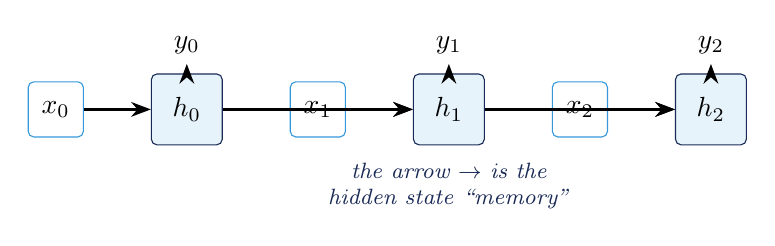
\begin{tikzpicture}[
  cell/.style={draw=primary, minimum size=0.9cm, rounded corners=2pt, fill=secondary!12},
  io/.style={draw=secondary, minimum size=0.7cm, rounded corners=2pt, fill=white},
  arr/.style={-{Stealth[length=2.5mm]}, thick}
]
\node[io] (x0) {$x_0$};
\node[cell, right=0.85cm of x0] (h0) {$h_0$};
\node[io, right=0.85cm of h0] (x1) {$x_1$};
\node[cell, right=0.85cm of x1] (h1) {$h_1$};
\node[io, right=0.85cm of h1] (x2) {$x_2$};
\node[cell, right=0.85cm of x2] (h2) {$h_2$};
\draw[arr] (x0) -- (h0);
\draw[arr] (h0) -- (h1);
\draw[arr] (x1) -- (h1);
\draw[arr] (h1) -- (h2);
\draw[arr] (x2) -- (h2);
\node[above=0.12cm of h0] (y0) {$y_0$}; \draw[arr] (h0) -- (y0);
\node[above=0.12cm of h1] (y1) {$y_1$}; \draw[arr] (h1) -- (y1);
\node[above=0.12cm of h2] (y2) {$y_2$}; \draw[arr] (h2) -- (y2);
\node[below=0.1cm of h1, align=center, font=\footnotesize\itshape, text=primary] {the arrow $\to$ is the\\ hidden state ``memory''};
\end{tikzpicture}
\end{center}

Think of it as passing a whispered note down a line of friends: each friend
reads the new word ($x_t$), updates the note ($h_t$), and passes it on.

\subsubsection{The Whisper Game Problem: Vanishing Gradients}

Remember the game ``telephone'' where a whisper gets quieter and quieter down
the line until the last person hears nothing? That is exactly what happens
during training with a simple RNN, called the \textbf{vanishing gradient}
problem.

To learn, the AI sends a ``how wrong was I?'' signal backwards through time
(\textbf{Backpropagation Through Time}). Each step multiplies that signal by
the hidden knob $W_{hh}$. If that knob is a bit less than 1, multiplying many
times makes the signal \emph{vanish} to almost zero --- the early steps learn
nothing. If the knob is a bit more than 1, the signal \emph{explodes} to
infinity. Either way, long-range memory fails. And multi-stage attacks NEED
long memory.

Simple RNNs are bad at remembering something from 20 windows ago. We need a
better notebook.

\subsection{3.3 LSTM: The Smart Notebook with Gates (Doors)}
\label{sec:lstm}

The \textbf{Long Short-Term Memory (LSTM)}, invented in 1997, fixes the whisper
problem with a brilliant idea: carry a separate \textbf{cell state} $c_t$ that
acts like a \textbf{conveyor belt / highway} through time, with little
\textbf{gates (doors)} that control what gets on and off.

\begin{imaginebox}
Picture a factory conveyor belt ($c_t$) carrying a notebook.

\begin{itemize}[leftmargin=1.6em,itemsep=1pt]
  \item A \textbf{Forget Gate} is a door that can throw some pages away.
  \item An \textbf{Input Gate} is a door that can add new pages.
  \item An \textbf{Output Gate} is a door that decides what to read out loud
        to the world ($h_t$).
\end{itemize}

Because the belt mostly just \emph{carries} the notebook with tiny edits (add
some, erase some), the ``how wrong was I'' signal can travel far without
vanishing. Long memory is saved!
\end{imaginebox}

Here are the six equations --- I will tell you the story of each one. Don't
memorise symbols; understand the \emph{job} each gate does.

Let $x_t$ be the new window, $h_{t-1}$ the previous read-out, and $[h_{t-1}, x_t]$
just means ``glue them together into one long list.''

\textbf{1. Forget Gate} --- ``How much of the old notebook should I keep?''
\[
f_t = \sigma\big( W_f [h_{t-1}, x_t] + b_f \big)
\]
$\sigma$ squishes to 0--1. So $f_t$ is a list of numbers like $[0.9, 0.1, 0.8]$
meaning ``keep 90\% of page 1, only 10\% of page 2 \dots'' 0 = forget fully,
1 = remember fully.

\textbf{2. Input Gate} --- ``How much new info should I let in?''
\[
i_t = \sigma\big( W_i [h_{t-1}, x_t] + b_i \big)
\]
Same idea: a 0--1 mask for how much of the new candidate to write.

\textbf{3. Candidate} --- ``What new stuff COULD I write?''
\[
\tilde{c}_t = \tanh\big( W_c [h_{t-1}, x_t] + b_c \big)
\]
This is the \emph{actual new content} proposed, squished to $-1$ to $1$.

\textbf{4. Update the Notebook} --- ``Make the edit.''
\[
c_t = f_t \odot c_{t-1} + i_t \odot \tilde{c}_t
\]
Keep some old ($f_t \odot c_{t-1}$) PLUS add some new ($i_t \odot \tilde{c}_t$).
Remember $\odot$ means multiply matching items. This is the highway!

\textbf{5. Output Gate} --- ``What should I show the world?''
\[
o_t = \sigma\big( W_o [h_{t-1}, x_t] + b_o \big)
\]

\textbf{6. New Read-Out} --- ``Read a cleaned-up version of the notebook aloud.''
\[
h_t = o_t \odot \tanh(c_t)
\]

\begin{keybox}
If the equations feel heavy, just remember the \textbf{notebook story}:
\emph{Forget some pages, write some new pages, read some pages aloud.} That is
all an LSTM does, 100 times per second. The cell $c_t$ is the notebook, $h_t$
is what you read aloud.
\end{keybox}

\subsection{3.4 GRU: The Lighter Backpack}
\label{sec:gru}

The \textbf{Gated Recurrent Unit (GRU)}, from 2014, is LSTM's simpler sibling.
It merges ``forget'' and ``input'' into one door called the \textbf{update
gate}, and it uses the read-out $h_t$ directly as the memory (no separate
notebook). Fewer knobs, faster, often just as good.

\begin{itemize}[leftmargin=1.6em,itemsep=2pt]
  \item \textbf{Reset Gate} $r_t = \sigma(W_r [h_{t-1}, x_t] + b_r)$:
        ``How much old memory should I ignore when making a new draft?''
  \item \textbf{Update Gate} $z_t = \sigma(W_z [h_{t-1}, x_t] + b_z)$:
        ``How much of the new draft should I actually use?''
  \item \textbf{Candidate}
        $\tilde{h}_t = \tanh(W_h [r_t \odot h_{t-1}, x_t] + b_h)$:
        the new draft (old memory first filtered by $r_t$).
  \item \textbf{Blend}
        $h_t = (1 - z_t) \odot h_{t-1} + z_t \odot \tilde{h}_t$:
        Mix old and new. If $z_t$ is near 0, keep the old. If near 1, adopt the
        new draft. Like fading between two photos.
\end{itemize}

\begin{keybox}
\textbf{Which should YOU use first?} Start with \textbf{GRU or LSTM}. They are
simple, well-tested, train fast on modest data, and beat fancier models surprisingly
often. Save Transformers for when you have lots of data and want long-range
spotlight attention.
\end{keybox}

\begin{yourturn}
Cover the ``meaning'' column for the LSTM gates and try to explain each gate's
job in your own words to an imaginary 12-year-old. If you can do it without
peeking, you own it. Then answer: why is $c_t$ called a ``highway''?
\end{yourturn}

\subsection{3.5 Transformers and Self-Attention: The Spotlight}
\label{sec:transformer}

\subsubsection{Why Another Model If LSTMs Work?}

LSTMs read time like a book: page 1, then page 2, then page 3, one by one.
That is slow (can't parallelise easily) and the link between page 1 and page
100 is still a long chain.

\textbf{Transformers} read the WHOLE book \emph{at once} and use a trick called
\textbf{self-attention} to let any page directly look at any other page. The
distance between page 1 and page 100 is one hop, not 99 hops. That is powerful
for spotting a scan 20 windows ago that relates to a theft now.

\subsubsection{The Spotlight Analogy}

\begin{imaginebox}
Imagine a classroom. The teacher asks: ``Who knows the answer?'' Each student
(student = one time window) has:

\begin{itemize}[leftmargin=1.6em,itemsep=1pt]
  \item A \textbf{Question} they are asking: ``I need info about scans.'' This
        is the \textbf{Query} ($q$).
  \item A \textbf{Label} on their desk: ``I have scan info / I have exfil info.''
        This is the \textbf{Key} ($k$).
  \item \textbf{Knowledge} in their head: the actual info they know. This is the
        \textbf{Value} ($v$).
\end{itemize}

When student $i$ wants to answer, they compare their Question ($q_i$) to every
other student's Label ($k_j$). The better the match, the brighter the
\textbf{spotlight} ($ \alpha_{ij}$) shines on that other student's Knowledge
($v_j$). The final answer for student $i$ is a weighted mix of everyone's
knowledge, with brighter spotlights counting more.

That, literally, is self-attention.
\end{imaginebox}

In maths:
\[
q_i = W_Q x_i,\qquad k_i = W_K x_i,\qquad v_i = W_V x_i
\]
\[
\text{score}(i,j) = \frac{q_i^\top k_j}{\sqrt{d_k}}\quad\text{(how well $i$'s question matches $j$'s label)}
\]
\[
\alpha_{ij} = \text{softmax}_j(\text{score}(i,j))\quad\text{(turn scores into spotlight brightnesses that sum to 1)}
\]
\[
\text{out}_i = \sum_j \alpha_{ij}\, v_j\quad\text{(mix everyone's knowledge by spotlight)}
\]

The $\sqrt{d_k}$ just stops numbers from getting too huge and confusing the
softmax (like dimming a blinding spotlight to a comfortable level).

\begin{examplebox}
\textbf{A sentence explains it best:}

``The cat chased the dog because \emph{it} was scared.''

Who is ``it''? Self-attention lets ``it'' shine its spotlight on ``dog'' more
than on ``cat.'' In network terms, it lets the model decide: ``This
exfiltration spike at window 50 is related to that SYN burst at window 30,
not to the normal web traffic at window 49.''
\end{examplebox}

\subsubsection{Multiple Spotlights and Page Numbers}

\begin{itemize}[leftmargin=1.6em,itemsep=2pt]
  \item \textbf{Multi-head attention} = run several spotlights in parallel,
        each with its OWN $W_Q, W_K, W_V$. One head might learn to watch
        \emph{ports}, another to watch \emph{timing}. Then glue their answers
        together. More eyes, more patterns.

  \item \textbf{Positional encoding} = Because attention looks at all pages at
        once, it has \emph{no idea about order} by itself. So we add a tiny
        number pattern (a ``page number'' written in invisible ink) to each
        input:
        \[
        PE_{(pos, 2i)} = \sin\!\Big(\frac{pos}{10000^{2i/d}}\Big),\qquad
        PE_{(pos, 2i+1)} = \cos\!\Big(\frac{pos}{10000^{2i/d}}\Big)
        \]
        Modern time-series Transformers sometimes use fancier clocks
        (``time2vec'') that also encode time-of-day or periodicity.
\end{itemize}

\subsubsection{The Transformer Block = LEGO Brick}

One block = \textbf{Multi-Head Attention} $\to$ add \& normalise $\to$
\textbf{Feed-Forward} (a small normal network) $\to$ add \& normalise. Stack
several blocks. For forecasting, feed $H$ past windows, predict the next $K$.

\begin{warnbox}
\textbf{Attention alone is NOT a prediction.} It is just the spotlight. You
still need a \emph{task head}: a small final layer that turns the spotlighted
mix into an actual answer (e.g., ``stage = C2 with 90\%''), plus a
\emph{loss} to train it (like cross-entropy for ``which stage?''). Don't
mistake the spotlight for the whole torch!
\end{warnbox}

\subsection{3.6 Dreaming K Steps Ahead: The Rollout}
\label{sec:rollout}

Now put it together. Given today's snapshot $S_t$, the \textbf{prediction
engine}:

\begin{enumerate}[leftmargin=1.8em,itemsep=2pt]
  \item \textbf{Encodes} the now.
  \item \textbf{Dreams} forward $K$ steps: predicts $S_{t+1}$, feeds that
        prediction back in as if it were real, predicts $S_{t+2}$, and so on up
to $S_{t+K}$. Like writing a story one sentence at a time, using your
own last sentence as the prompt for the next.
  \item \textbf{Collects} the dream into three human outputs:
        \begin{enumerate}[label=\alph*.,leftmargin=1.6em]
          \item \textbf{Probability timeline}: how likely is trouble in each of
the next $K$ windows? Example: $[0.1, 0.3, 0.7, 0.85, 0.9]$
(getting worse).
          \item \textbf{Stage trajectory}: which ATT\&CK stage at each step?
Example: Recon $\to$ Recon $\to$ Initial Access $\to$ C2.
          \item \textbf{Reasons}: why does the model think so? (SHAP + attention,
next chapter).
        \end{enumerate}
\end{enumerate}

\subsubsection{Teacher Forcing vs.\ Real Dreaming}

\begin{itemize}[leftmargin=1.6em,itemsep=2pt]
  \item \textbf{Teacher forcing (training):} Feed the \emph{real} next step as
        input, even if the model's own prediction was wrong. Like a teacher
whispering the correct next word during practice. Learns fast, but
never practises recovering from its own mistakes.

  \item \textbf{Autoregressive rollout (real life):} Feed the model's \emph{own}
last prediction as the next input. This is how it will actually run,
but mistakes can \emph{compound}: a small error at step 1 becomes a
bigger error at step 5. We often \emph{mix} both during training
(called \textbf{scheduled sampling}) so the model learns to be robust.
\end{itemize}

\begin{warnbox}
Because errors stack, keep $K$ \emph{modest} (maybe 5--10 windows), report
scores \emph{per step} (``step-1 accuracy, step-5 accuracy'') not just one
number, and show how confidence fades further into the future. Honesty builds
trust.
\end{warnbox}

\subsection{3.7 Graph Neural Networks: The Social Network of Computers}
\label{sec:gnn}

So far, we treated windows as lists. But a network is really a \textbf{social
network}: computers are \emph{people} (nodes), and flows are \emph{friendships}
(edges). That shape matters! A scanner talks to \emph{many} strangers
(one-to-many). A server that is being DDoS'd is talked to \emph{by many} people
(many-to-one). That shape IS a clue.

\begin{center}
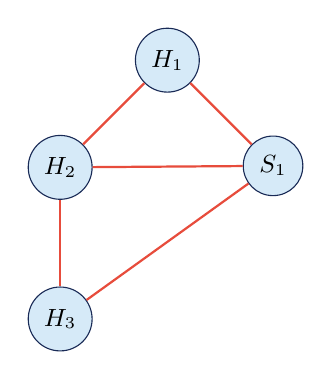
\begin{tikzpicture}[
  node/.style={draw=primary, fill=secondary!20, circle, minimum size=0.7cm, font=\small},
  edge/.style={draw=accent, thick}
]
\node[node] (a) {$H_1$};
\node[node, below left=1.1cm of a] (b) {$H_2$};
\node[node, below right=1.1cm of a] (c) {$S_1$};
\node[node, below=1.1cm of b] (d) {$H_3$};
\draw[edge] (a) -- (b); \draw[edge] (a) -- (c); \draw[edge] (b) -- (c);
\draw[edge] (b) -- (d); \draw[edge] (c) -- (d);
\end{tikzpicture}
\end{center}

\subsubsection{Gossip as Maths: Message Passing}

How do GNNs work? Like \textbf{gossip}. Each person (node) listens to their
neighbours, mixes what they hear with what they already know, and updates their
own story. Do this layer by layer, and after a few rounds each person knows a
bit about the whole town.

For node $v$ at layer $\ell$:
\[
h_v^{(\ell+1)} =
\text{UPDATE}\Big( h_v^{(\ell)},\ \text{AGGREGATE}\big(\{ h_u^{(\ell)} : u \in \mathcal{N}(v) \}\big) \Big)
\]

In words: ``My new story = combine (my old story, the combined story of all
my neighbours).'' AGGREGATE is usually an average or a sum. UPDATE is a small
neural net.

Popular flavours:
\begin{itemize}[leftmargin=1.6em,itemsep=2pt]
  \item \textbf{GCN} (Graph Convolutional Network): neighbour average, with a
        neat normalisation.
  \item \textbf{GAT} (Graph Attention Network): neighbours don't count equally;
        the model learns \emph{who to listen to more} (attention on the graph).
  \item \textbf{GraphSAGE}: samples a few neighbours so it scales to huge towns.
  \item \textbf{GIN}: very expressive for telling different shapes apart.
\end{itemize}

\subsubsection{GCN in One Line (Don't Fear It)}

\[
h_v^{(\ell+1)} = \sigma\!\Bigg( W^{(\ell)}\,
\sum_{u \in \mathcal{N}(v) \cup \{v\}}
\frac{1}{\sqrt{\deg(u)\,\deg(v)}}\ h_u^{(\ell)} \Bigg)
\]

Translation: ``Average my neighbours' stories and my own, but divide by how
popular each person is so a super-popular person doesn't dominate. Then turn
the knob $W$ and squish with $\sigma$.'' That division is just to keep numbers
well-behaved.

\subsubsection{Time + Graph = Spatio-Temporal}

Because we have time \emph{and} a graph, we combine them:
\begin{itemize}[leftmargin=1.6em,itemsep=2pt]
  \item \textbf{ST-GCN}: do a graph gossip step, then a time step (1D
        convolution), repeat. Like alternating between ``who talks to whom''
        and ``how things change over time.''
  \item \textbf{GNN + LSTM/Transformer}: GNN makes a good summary of the
        \emph{town shape} at each time slice; then an LSTM/Transformer watches
the \emph{movie} of those summaries.
\end{itemize}

\begin{tipbox}
\textbf{Where to start?} Don't build a huge graph on day one. For your first
prototype, build a simple \textbf{host graph} per window (nodes = computers,
edges = flows seen in that window), run a tiny GCN to get a shape summary,
and feed that sequence into a GRU. Simple, explainable, and judges will love
that you thought about topology.
\end{tipbox}

\begin{recap}
\textbf{Chapter 3 recap:} A World Model is a \emph{forecaster}, not just a
classifier: it learns $P(S_{t+1}\mid S_t)$ and dreams $K$ steps ahead. LSTMs
carry a notebook with gates to remember far back; GRUs are the lighter version;
Transformers use spotlights (attention) to connect far-apart pages; and GNNs
add the social-network shape via gossip (message passing). Layer them to build
your dream machine.
\end{recap}

\newpage

% ===========================================================================
% CHAPTER 4
% ===========================================================================
\section{Chapter 4: Making AI Explain Itself \\
\small Interpretability \& Explainable AI (XAI)}
\label{sec:xai}

\subsection{4.1 Why ``Trust Me, I'm AI'' Is Not Enough}

Your challenge says, in bold: \emph{``Black-box models are unacceptable.''}
You MUST include an \textbf{Explainability Engine} that turns ``the AI said
so'' into ``here is \emph{why} the AI said so, in words a human can check.''

Why? Imagine a doctor says ``You need surgery'' but refuses to say why. Would
you trust them? A security analyst feels the same about an AI that just shouts
``ATTACK!'' with no reason. Explainability builds \textbf{trust}, lets you
\textbf{debug} mistakes, and impresses judges.

Two questions matter:

\begin{enumerate}[leftmargin=1.8em,itemsep=2pt]
  \item \textbf{``Which clues (features) made the difference?''}
        Was it the many SYNs? The weird port? The fast timing? $\to$ Answer:
        \textbf{SHAP}.

  \item \textbf{``Which time slices did the model stare at?''}
        Did it look at the scan 20 windows ago or just the last one?
        $\to$ Answer: \textbf{attention weights}.
\end{enumerate}

One tells you \emph{what} mattered, the other \emph{when/where}.

\subsection{4.2 SHAP: Fairly Sharing Credit (The Pizza Party)}
\label{sec:shap}

\subsubsection{The Pizza Party That Explains Everything}

\begin{storybox}
Five friends order a pizza together. The bill is \$50. But the fun they had
depends on \emph{who came}. Alice alone is quiet, but Alice + Bob together are
hilarious. How do you fairly say ``Alice contributed this much to the fun,
Bob this much \dots'' when the value depends on the \emph{group}?

\textbf{Lloyd Shapley}, a mathematician, proved there is ONE fair way: for each
person, look at \emph{every possible group} they could join, see how much the
group's fun \emph{increases} when they join, and average that over all groups.
That average increase is their \textbf{Shapley value}.

In AI: the ``friends'' are your \textbf{features}, the ``fun'' is the
\textbf{prediction} (e.g., 0.92 = ``probably an attack''). SHAP does the same
fair averaging to say ``Feature `many SYNs' pushed the prediction up by +0.25.''
\end{storybox}

\begin{keybox}
\textbf{Shapley value} = a feature's \emph{average} extra contribution to the
prediction, averaged over every possible combination of other features. SHAP
makes this practical with a clever \emph{additive} trick so you don't have to
try literally every combination (which would take forever).
\end{keybox}

\subsubsection{The Additive Sentence}

SHAP writes the explanation as a simple sum:

\[
g(x') = \phi_0 + \sum_{i=1}^{M} \phi_i \ x'_i
\]

In English:

\begin{itemize}[leftmargin=1.6em,itemsep=2pt]
  \item $x'_i$ is 1 if feature $i$ is ``present,'' 0 if ``absent'' (like
        ``is Alice at the party?'' yes/no).
  \item $\phi_0$ is the \textbf{baseline}: the average prediction over all
examples (like ``on a random day, the AI says 10\% chance of attack'').
  \item $\phi_i$ is the \textbf{SHAP value} for feature $i$: how much that
feature pushed the prediction away from baseline for \emph{this}
specific example.
  \item $g(x')$ should be close to the real model output $f(x)$ for this
example (local accuracy).
\end{itemize}

\subsubsection{How to Read a SHAP Value (Like Reading a Report Card)}

\begin{itemize}[leftmargin=1.6em,itemsep=2pt]
  \item \textbf{Positive $\phi_i$} (e.g., +0.30) = this feature pushed the
answer \emph{UP} toward ``attack.''
  \item \textbf{Negative $\phi_i$} (e.g., $-0.20$) = this feature pulled it
\emph{DOWN} toward ``benign.''
  \item \textbf{Big absolute value} = very important for this decision.
  \item \textbf{Small near zero} = didn't matter much this time.
\end{itemize}

\begin{examplebox}
\textbf{A real reading:}

The AI says ``attack with 92\% chance.'' The average (baseline) is only 10\%.
So it moved $+0.82$ above baseline. Why?

\[
\phi(\text{weird dst port}) = +0.30,\qquad
\phi(\text{high SYN count}) = +0.25
\]
\[
\phi(\text{very short gaps between packets}) = +0.15
\]

Now a human analyst reads: ``Ah, it flagged because of the port, the many
hellos, and the burstiness. That matches a scan.'' \emph{Explainable!}
\end{examplebox}

\subsubsection{SHAP in Python (You Don't Need to Code This From Scratch)}

\begin{lstlisting}[language=Python]
import shap

# 1. Make an explainer for your trained model.
explainer = shap.TreeExplainer(model)      # for tree models; exact and fast

# 2. Ask it to explain some examples.
shap_values = explainer.shap_values(X_sample)

# 3. Draw pictures.
shap.summary_plot(shap_values, X_sample)   # which features matter overall?
shap.force_plot(explainer.expected_value, shap_values[0], X_sample.iloc[0])
                                           # why this ONE example?
\end{lstlisting}

Which explainer to pick?
\begin{itemize}[leftmargin=1.6em,itemsep=2pt]
  \item \textbf{TreeExplainer} --- for tree models (Random Forest, XGBoost).
        Exact, fast. Great for baselines.
  \item \textbf{Gradient / DeepExplainer} --- for neural nets (LSTM,
        Transformer). Uses gradients (the learning signal).
  \item \textbf{KernelExplainer} --- works with ANY model but is slow; use on
a few examples only.
  \item \textbf{LinearExplainer} --- for simple linear models.
\end{itemize}

\begin{warnbox}
SHAP is \textbf{per-example} and \textbf{model-specific}. For your
sequence model, explain the \emph{final input window's feature vector} (the
thing that went into the last prediction head), not the raw packets. And always
remember: SHAP explains what the \emph{model} did, not necessarily what is
true in the real world.
\end{warnbox}

\subsection{4.3 Attention Weights: Peeking Over the AI's Shoulder}
\label{sec:attention}

\subsubsection{What Are They?}

In a Transformer, the spotlight brightnesses $\alpha_{ij}$ say: ``When making
the answer for position $i$, how much did I look at position $j$?'' If you
save those numbers, you can literally see \emph{where the model was looking}.

\begin{keybox}
\textbf{SHAP} = ``\emph{which clues} mattered'' (the what).\\
\textbf{Attention} = ``\emph{which time slices} the model stared at'' (the when).

Use both. They answer different questions, and judges love seeing both in a
demo.
\end{keybox}

\subsubsection{How to Get Them in Code}

During the forward pass (the prediction), the Transformer computes attention
inside. You just save it:

\begin{lstlisting}[language=Python]
# In PyTorch, after a forward pass:
attn_weights = model.get_attention(input_window)  # shape: [heads, time, time]
# attn_weights[h, i, j] = how much head h, at time i, looked at time j
\end{lstlisting}

In many libraries you can add a \texttt{hook} (a little spy) that saves the
tensor without changing training code at all.

\subsubsection{The Heatmap (The Picture Judges Remember)}

Make an $n \times n$ coloured grid: rows = ``who is asking'' (query time),
columns = ``who is being looked at'' (key time), colour = brightness.

What you usually see:
\begin{itemize}[leftmargin=1.6em,itemsep=2pt]
  \item A bright \textbf{diagonal}: each moment mostly looks at itself and
        neighbours (natural).
  \item Occasional bright \textbf{off-diagonal spots}: a far-away moment that
mattered a lot (e.g., a scan 20 windows ago suddenly relevant now).
Those spots are the \emph{long-range connections} your World Model
learned --- point them out in your demo!
\end{itemize}

\begin{warnbox}
Research warns: attention is a \emph{useful signal}, not a \emph{proof}.
A model can attend to something without truly using it, or use something
without attending strongly. Treat attention as \emph{evidence}, combine it with
SHAP, and you will be honest and strong.
\end{warnbox}

\begin{tipbox}
\textbf{Demo gold:} On one screen, show: (1) the probability timeline going
up, (2) the predicted ATT\&CK colours per window, (3) the attention heatmap
with circles on the key spots, and (4) a SHAP bar chart saying ``flagged
because: many SYNs, weird port, burst timing.'' That is end-to-end
explainability. Judges will applaud.
\end{tipbox}

\begin{recap}
\textbf{Chapter 4 recap:} Black boxes are not allowed. SHAP fairly shares
credit among features (like sharing pizza bill fairly). Attention shows where
in time the model looked. Together they turn ``Trust me'' into ``Here's why,
check it yourself.''
\end{recap}

\newpage

% ===========================================================================
% CHAPTER 5
% ===========================================================================
\section{Chapter 5: Turning It Into a Real Product \\
\small Deployment, Benchmarking \& Systems}
\label{sec:deploy}

So you built a World Model that can dream. How do you turn that lab experiment
into a \emph{real thing} someone can download, run offline, and trust? And how
do you \emph{prove} it is better than the simple thing?

\subsection{5.1 Building an Offline Product (No Internet Needed)}
\label{sec:offline}

Your challenge requires a \textbf{fully open-source, fully offline} product.
No calling ChatGPT, no cloud. Everything must run on the judge's laptop with
no Wi-Fi. That shapes every choice.

\subsubsection{The Six Pieces You Must Deliver (The Check-list)}

\begin{enumerate}[leftmargin=1.8em,itemsep=2pt]
  \item \textbf{Feature Extraction Pipeline} --- the code that turns a raw
        PCAP or CSV into the clean, normalised table of numbers (the feature
        matrix) with timestamps. This is the kitchen that prepares ingredients.

  \item \textbf{Trained World Model} --- your actual AI: training scripts,
        saved knobs (weights), and a config file so anyone can reproduce your
training exactly.

  \item \textbf{Prediction Engine} --- the code that takes a fresh snapshot
$S_t$ and \emph{dreams} $K$ steps: $S_{t+1}\dots S_{t+K}$ plus
probabilities and stages.

  \item \textbf{Explainability Engine} --- the code that runs SHAP and grabs
attention maps to list \emph{driving features} in human words.

  \item \textbf{Demo Interface} --- an \textbf{offline} app a judge can double
click: maybe \textbf{Streamlit} (pretty web app), \textbf{Flask}, or
even a simple \textbf{CLI} (text menu). It must: accept a PCAP/CSV,
run the whole pipeline, and show the timeline, flagged flows, and stage
colours. No internet.

  \item \textbf{Benchmark Results} --- a table proving you beat a simple
\textbf{logistic regression} on the \emph{same} features. Without this,
your claim is just words.
\end{enumerate}

\subsubsection{The Assembly Line (How Data Flows Through Your Product)}

\[
\underbrace{\texttt{PCAP / CSV}}_{\text{input file}}
\ \xrightarrow{\text{Feature Extraction}}\ 
\underbrace{X_{\text{windows}}}_{\text{save this!}}
\]
\[
\underbrace{X_{\text{windows}}}_{\text{cached}} \ \xrightarrow{\text{World Model}}\ 
\underbrace{\text{dream} \to \text{stages + scores}}_{\text{predictions}}
\ \xrightarrow{\text{XAI (SHAP + attn)}}\ 
\underbrace{\text{human reasons}}_{\text{demo}}
\]

Keep each arrow as a separate function/class so you can test and swap pieces
without breaking everything (like LEGO, not like a tangled knot of wires).

\begin{tipbox}
\textbf{Speed matters in a live demo.} Parsing a big PCAP can take minutes.
\textbf{Cache} (save) the feature matrix to a file after the first run so the
second run is instant. Also log the dataset filename and a hash (like
\texttt{sha256}) so you can prove ``this demo ran on exactly this file,
these features.''
\end{tipbox}

\subsection{5.2 How Do We Know It's Good? Measuring with Honest Numbers}
\label{sec:benchmark}

\subsubsection{Your Opponent: The Simple Baseline}

The challenge says you must beat:

\[
\text{baseline} = \text{logistic regression trained on the SAME features}
\]

What is \textbf{logistic regression}? Just the simplest sensible AI: draw a
straight line (well, a gentle S-curve) to separate benign from attack. If your
fancy World Model can't beat this simple line, something is wrong.

\emph{Same features} is the key: both models must see the \emph{same} windowed
table. Otherwise you are not comparing AIs, you are comparing kitchens.

\subsubsection{The Four Numbers That Matter (Meet the Confusion Matrix)}

Forget ``accuracy'' for a minute. On security data it lies (we will see why).
Instead, imagine we test on 100 examples and count:

\begin{center}
\small
\begin{tabular}{@{}c|cc@{}}
      & \textbf{AI says Attack} & \textbf{AI says Benign} \\
\midrule
\textbf{Really Attack} & TP (True Positive) = caught & FN (False Negative) = missed \\
\textbf{Really Benign} & FP (False Positive) = false alarm & TN (True Negative) = correctly ignored \\
\end{tabular}
\end{center}

Now the four scores, with a tiny example: Suppose TP=80, FN=20, FP=10, TN=90.

\begin{itemize}[leftmargin=1.6em,itemsep=2pt]
  \item \textbf{Precision} $= \dfrac{TP}{TP+FP} = \dfrac{80}{80+10}=0.89$:

        ``When my alarm rang, how often was it REAL?''
        High precision = few false alarms. Low precision = you cry wolf and
        analysts stop listening.

  \item \textbf{Recall} $= \dfrac{TP}{TP+FN} = \dfrac{80}{80+20}=0.80$:

        ``Of all real attacks, how many did I catch?''
        High recall = you rarely miss a burglar. Low recall = burglars slip
        through.

  \item \textbf{F1} $= 2\cdot\dfrac{precision\cdot recall}{precision+recall}$:

The harmonic mean (a balanced blend) of the two. If either is low, F1
is low. With 0.89 and 0.80, F1 $\approx 0.84$.

  \item \textbf{False Positive Rate (FPR)} $= \dfrac{FP}{FP+TN}
= \dfrac{10}{10+90}=0.10$:

        ``How often do I falsely accuse innocent traffic?'' In security, high
        FPR is deadly --- analysts burn out and ignore your tool.
\end{itemize}

\begin{warnbox}
\textbf{Why accuracy fools you:}
Imagine 99 of 100 examples are benign, 1 is attack. A lazy AI that always says
``benign'' gets accuracy $= 99/100 = 99\%$! It looks amazing but caught ZERO
attacks. Precision/recall/F1 expose this trick. On imbalanced data, \textbf{never
lead with accuracy}.
\end{warnbox}

\subsubsection{Extra Scores for Forecasting (You Are a Forecaster, Remember)}

\begin{itemize}[leftmargin=1.6em,itemsep=2pt]
  \item \textbf{Per-step scores}: F1 at step 1, step 2, \dots\ step K. Step-1 is
usually high, step-K fades. Showing the fade is honest and expected.

  \item \textbf{AUC-ROC / AUC-PR}: how well you \emph{rank} examples without
picking a threshold. AUC-PR is better when attacks are rare (imbalanced).

  \item \textbf{Calibration / Brier score}: ``When you say 80\% chance, does it
actually happen 80\% of the time?'' Good calibration means your
percentages are trustworthy.

  \item \textbf{Stage-accuracy}: ``How often did you get the ATT\&CK stage right?''
(Recon vs.\ C2 etc.).
\end{itemize}

\subsubsection{The Honest Benchmark Recipe (Do This Exactly)}

\begin{enumerate}[leftmargin=1.8em,itemsep=2pt]
  \item \textbf{Split by time}, leakage-free (Chapter 2.3).
  \item \textbf{Fit scalers on train only} (Chapter 2.3).
  \item Train \textbf{both} the simple baseline AND your World Model on the
\emph{identical} feature table.
  \item Test both on the \emph{same} held-out future timeline.
  \item Report precision, recall, F1, FPR \emph{per horizon step} (not one
blurry number).
  \item Sanity-check with a \textbf{random guesser} and a \textbf{plain LSTM}
so you know your gain is real, not luck.
\end{enumerate}

\begin{examplebox}
\textbf{How your benchmark table should look:}

\begin{center}
\small
\begin{tabular}{@{}lcccc@{}}
\toprule
Model & Precision & Recall & F1 & FPR \\
\midrule
Random Guessing & 0.50 & 0.50 & 0.50 & 0.50 \\
Logistic Regression (required baseline) & 0.78 & 0.62 & 0.69 & 0.05 \\
LSTM World Model (K=5) & 0.86 & 0.79 & 0.82 & 0.03 \\
Temporal Transformer & 0.90 & 0.85 & 0.87 & 0.02 \\
GNN + GRU & 0.88 & 0.86 & 0.87 & 0.02 \\
\bottomrule
\end{tabular}
\end{center}

On one dataset these are point estimates. Use time-fold cross-validation and
report ranges if you can. And say which metric you optimised for (often F1
or AUC-PR, not accuracy).
\end{examplebox}

\subsection{5.3 The Full Journey: Your 10-Step Roadmap}
\label{sec:workflow}

Tape this to your wall:

\begin{enumerate}[leftmargin=1.8em,itemsep=2pt]
  \item \textbf{Ingest} --- load CIC-IDS CSV (or parse PCAP with Scapy).
  \item \textbf{Make features} --- flow + packet clues (Chapter 1.6).
  \item \textbf{Slice time} --- cut into $H$-length window histories, label each
        window (Chapter 1.10).
  \item \textbf{Split honestly} --- by time, no leakage (Chapter 2.3).
  \item \textbf{Train the World Model} --- GRU/LSTM/Transformer/GNN+GRU;
        pick your encoder + dynamics head; walk-forward validate.
  \item \textbf{Dream forward} --- K-step rollout $\to$ scores + stage path
        (Chapter 3.6).
  \item \textbf{Explain} --- attention + SHAP $\to$ driving features
        (Chapter 4).
  \item \textbf{Build the demo} --- Streamlit/Flask/CLI, offline, drag-and-drop
        PCAP/CSV $\to$ timeline + stages + attention + SHAP.
  \item \textbf{Benchmark} --- vs.\ logistic regression, with honest numbers
        (Chapter 5.2).
  \item \textbf{Package} --- source code on GitHub, README with setup steps,
        2-page architecture doc, \textless{}2 minute demo video,
        \textless{}5 slides.
\end{enumerate}

\begin{keybox}
\textbf{The One Sentence to Remember Forever:}

A World Model is not a classifier that says ``attack / not attack.'' It is a
\emph{simulator of the network through time}:

\begin{quote}
\emph{See} the state\ $\to$\ \emph{Learn} how it changes\ $\to$\ \emph{Dream}
$K$ steps ahead\ $\to$\ \emph{Name} the stage (ATT\&CK)\ $\to$\ \emph{Explain}
why (SHAP + attention)\ $\to$\ \emph{Prove} you're better than simple
(benchmark).
\end{quote}

Master this loop and you haven't just built a model --- you've built a
\emph{radar that sees the future}. That's a superpower.
\end{keybox}

\begin{recap}
\textbf{Chapter 5 recap:} Build offline and open-source. Prove you beat a
simple line (logistic regression) with precision/recall/F1 (not accuracy).
Keep every stage as LEGO bricks. Cache slow steps. And make your demo tell
\emph{the whole story}: timeline + stages + spotlight + reasons.
\end{recap}

\newpage

% ===========================================================================
% CONCLUSION
% ===========================================================================
\section*{A Final Word From Your Teacher --- You Did It!}
\addcontentsline{toc}{section}{A Final Word From Your Teacher}
\markboth{A Final Word}{}

Take a breath. Look how far you came.

On page 1, ``network telemetry'' might have sounded like a foreign language.
Now you know it is just ``measuring the letters on the roads and writing
report cards.'' On page 1, LSTM might have sounded scary. Now you see a little
notebook with three doors. That is real learning.

Here is the map of where you have been:

\begin{itemize}[leftmargin=1.6em,itemsep=2pt]
  \item \textbf{Chapter 0} gave you the ABCs: network = town, data = letters,
        AI = a baker who tastes and adjusts, $P$ = chance.
  \item \textbf{Chapter 1} taught you how letters travel (IP = house, port =
        door, TCP = polite call with SYN/ACK), how we summarise them into flows,
        how we cut time into windows, and how to read a PCAP line by line.
  \item \textbf{Chapter 2} taught you how burglars think (ATT\&CK = the
        playbook), where to get practice papers (CIC-IDS, CTU-13), and the
        golden rule: \emph{never let the future leak into the past}.
  \item \textbf{Chapter 3} taught you to make AI \emph{dream}: LSTMs with
        notebooks, GRUs as lighter backpacks, Transformers as spotlights, GNNs
        as gossip, and rollouts as dreaming $K$ steps ahead.
  \item \textbf{Chapter 4} taught you to make AI \emph{explain}: SHAP = fair
        pizza sharing, attention = where the spotlight shone.
  \item \textbf{Chapter 5} taught you to turn it into a real offline product
        and to prove it with honest numbers (precision/recall/F1, not accuracy).
\end{itemize}

A few last encouragements, from one builder to another:

\begin{itemize}[leftmargin=1.6em,itemsep=2pt]
  \item \textbf{Start simple.} A working GRU beats a broken 12-layer
        Transformer. Get one thing working, \emph{then} climb.

  \item \textbf{Trust honest numbers.} If your score looks like 99.9\%, check
        for leakage or imbalance first, not champagne. Honest 85\% beats
        cheating 99\% in front of a judge.

  \item \textbf{Explain everything.} A modest model that can say ``because
        many SYNs on port 4444'' beats a perfect black box that just says
        ``attack.'' Judges trust what they can see.

  \item \textbf{Show the movie, not just the snapshot.} Your demo should let a
        judge \emph{watch} the attack unfold stage by stage, with the attention
        spotlight and SHAP reasons side by side.

  \item \textbf{Have fun.} You are building something that could one day help
a real security team stop a real burglar. That's a beautiful, meaningful
thing to do. Be proud of it.
\end{itemize}

If you understood even 70\% of this book on the first read, you are ahead of
most beginners. Reread the chapters you found hard, do the ``Your Turn''
exercises with a friend, and run the code snippets on a small dataset. The
second read will feel like a different book --- an easy one.

Go build your World Model. I'm cheering for you, every step of the way.
\\[0.8em]
--- \emph{Your Teacher} \quad :) \\[0.6em]
{\small\textit{P.S. If a line still confuses you, read it out loud as if you
are explaining it to a 10-year-old. If you can explain it simply, you
understand it deeply. That's the Feynman trick --- and it works.}}

\newpage

% ===========================================================================
% APPENDICES
% ===========================================================================
\section*{Appendix A: Glossary --- Every New Word in One Place}
\addcontentsline{toc}{section}{Appendix A: Glossary}
\markboth{Appendix A: Glossary}{}

\begin{itemize}[leftmargin=1.4em,itemsep=1pt]
  \item \textbf{Accuracy} --- fraction of all predictions that were correct. Lies on imbalanced data.
  \item \textbf{ATT\&CK} --- the playbook of hacker tactics and techniques (MITRE).
  \item \textbf{Attention} --- spotlight that lets one time step focus on another.
  \item \textbf{Benign} --- normal, harmless traffic.
  \item \textbf{Bias ($b$)} --- a small nudge added in a neural net layer.
  \item \textbf{C2 (Command and Control)} --- hacker secretly talking to their server.
  \item \textbf{Cell state ($c_t$)} --- the notebook carried through time in an LSTM.
  \item \textbf{CIC-IDS / CTU-13} --- well-known practice datasets with labelled traffic.
  \item \textbf{Classifier} --- AI that says ``what is this?'' (one snapshot).
  \item \textbf{Dataset} --- folder of examples + answer keys.
  \item \textbf{Discretisation} --- turning smooth time into counted buckets.
  \item \textbf{Encapsulation} --- wrapping data layer by layer, like nested boxes.
  \item \textbf{Exfiltration} --- stealing data out.
  \item \textbf{Feature} --- one clue (number) the AI reads.
  \item \textbf{Feature vector} --- the list of all clues for one example.
  \item \textbf{Flow} --- summary (report card) of one conversation (same 5-tuple).
  \item \textbf{Flow record} --- one row in the flow table.
  \item \textbf{FPR} --- False Positive Rate: how often you falsely blame innocent traffic.
  \item \textbf{GAT / GCN / GNN} --- Graph Neural Network family; learns from town shape.
  \item \textbf{GRU} --- lighter LSTM with two gates (reset + update).
  \item \textbf{Hidden state ($h_t$)} --- AI's memory carried through time.
  \item \textbf{IP address} --- house address of a computer.
  \item \textbf{IPFIX / NetFlow} --- standard ways to write and export flow report cards.
  \item \textbf{Label} --- the correct answer for training (e.g., Benign/Bot).
  \item \textbf{Leakage} --- when future/test info sneaks into training (cheating).
  \item \textbf{LSTM} --- memory network with forget/input/output gates and a cell notebook.
  \item \textbf{PCAP} --- file of saved packets (box of saved letters).
  \item \textbf{Port} --- door number inside a house (e.g., 80 = web, 22 = SSH).
  \item \textbf{Precision} --- when you said ``attack,'' how often were you right?
  \item \textbf{Protocol} --- language inside (6=TCP, 17=UDP).
  \item \textbf{Recall} --- of all real attacks, how many did you catch?
  \item \textbf{RNN} --- Recurrent Neural Network; has memory over time.
  \item \textbf{Rollout} --- dreaming $K$ steps ahead, feeding each prediction back in.
  \item \textbf{Scaler} --- rescales numbers to a similar range (e.g., 0--1).
  \item \textbf{SHAP} --- fair way to share credit among features for one prediction.
  \item \textbf{SYN / ACK / FIN / RST} --- TCP verbs: hello / got it / goodbye / abort.
  \item \textbf{Telemetry} --- measuring from far away (here: measuring the network).
  \item \textbf{Transformer} --- AI that reads all time steps at once with attention.
  \item \textbf{TTL} --- countdown before a packet is thrown away (hops left).
  \item \textbf{Vector} --- ordered list of numbers.
  \item \textbf{Weight ($W$)} --- knob the AI turns to say how strongly to listen to a clue.
  \item \textbf{Window} --- one time slice (e.g., 60 seconds) summarised into a snapshot.
  \item \textbf{World Model} --- AI that learns how the world changes and dreams the future.
  \item \textbf{XAI} --- Explainable AI; making the AI say \emph{why} it decided.
\end{itemize}

% ---------------------------------------------------------------------------
\section*{Appendix B: Quick Reference --- Key Equations}
\addcontentsline{toc}{section}{Appendix B: Quick Reference}

\subsection*{RNN (the basic memory)}
\begin{equation*}
h_t = \tanh(W_{hh} h_{t-1} + W_{xh} x_t + b_h)
\end{equation*}

\subsection*{LSTM --- the six-gate notebook (jobs on the right)}
\begin{align*}
f_t &= \sigma(W_f [h_{t-1},x_t] + b_f) & \tilde{c}_t &= \tanh(W_c [h_{t-1},x_t] + b_c)\\
i_t &= \sigma(W_i [h_{t-1},x_t] + b_i) & o_t &= \sigma(W_o [h_{t-1},x_t] + b_o)\\
c_t &= f_t \odot c_{t-1} + i_t \odot \tilde{c}_t & h_t &= o_t \odot \tanh(c_t)
\end{align*}

\subsection*{GRU --- the lighter backpack}
\begin{align*}
r_t &= \sigma(W_r [h_{t-1},x_t] + b_r) & z_t &= \sigma(W_z [h_{t-1},x_t] + b_z)\\
\tilde{h}_t &= \tanh(W_h [r_t \odot h_{t-1}, x_t] + b_h) & h_t &= (1-z_t) \odot h_{t-1} + z_t \odot \tilde{h}_t
\end{align*}

\subsection*{Self-Attention (the spotlight)}
\begin{equation*}
\text{out}_i = \text{softmax}_j\!\Big(\frac{q_i^\top k_j}{\sqrt{d_k}}\Big)\, v_j
\end{equation*}

\subsection*{GCN (gossip on the graph)}
\begin{equation*}
h_v^{(\ell+1)} = \sigma\Big( W^{(\ell)}
\textstyle\sum_{u \in \mathcal{N}(v)\cup\{v\}}
\frac{h_u^{(\ell)}}{\sqrt{\deg(u)\deg(v)}} \Big)
\end{equation*}

\subsection*{SHAP additive explanation}
\begin{equation*}
g(x') = \phi_0 + \sum_{i=1}^{M} \phi_i \, x'_i
\end{equation*}

\subsection*{World Model dynamics}
\begin{equation*}
P(S_{t+1} \mid S_t)
\end{equation*}

\subsection*{Metrics}
\begin{align*}
\text{Precision} &= \frac{TP}{TP+FP}, &
\text{Recall} &= \frac{TP}{TP+FN}\\[0.3em]
\text{F1} &= \frac{2\,PR}{P+R}, &
\text{FPR} &= \frac{FP}{FP+TN}
\end{align*}

\subsection*{Flow Feature Checklist (What to Compute Per Flow)}
\begin{itemize}[leftmargin=1.6em,itemsep=1pt]
  \item 5-tuple: src/dst IP, src/dst port, protocol.
  \item Byte / packet counts (total, forward, reverse).
  \item Duration; flow bytes/s; flow packets/s.
  \item IAT stats: min, max, mean, std (forward + backward).
  \item Packet-size stats: min, max, mean, std.
  \item TCP flag counts (SYN, ACK, PSH, RST, FIN).
  \item Active / idle time stats.
  \item Packet-level extras: TTL variance, window size, fragment flags, retransmissions.
\end{itemize}

% ---------------------------------------------------------------------------
\section*{Appendix C: The Five Forecast Stages}
\addcontentsline{toc}{section}{Appendix C: The Five Forecast Stages}

\begin{center}
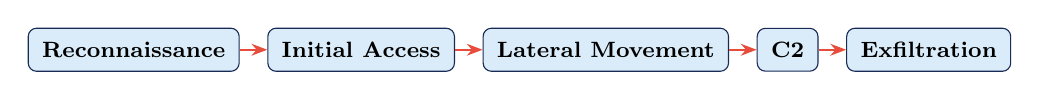
\begin{tikzpicture}[
  st/.style={draw=primary, fill=secondary!18, rounded corners=3pt,
    minimum height=0.5cm, inner sep=5pt, font=\footnotesize\bfseries},
  ar/.style={-{Stealth[length=2mm]}, thick, color=accent}
]
\node[st] (r) {Reconnaissance};
\node[st, right=0.35cm of r] (i) {Initial Access};
\node[st, right=0.35cm of i] (l) {Lateral Movement};
\node[st, right=0.35cm of l] (c) {C2};
\node[st, right=0.35cm of c] (e) {Exfiltration};
\draw[ar] (r) -- (i); \draw[ar] (i) -- (l);
\draw[ar] (l) -- (c); \draw[ar] (c) -- (e);
\end{tikzpicture}
\end{center}

\noindent This is the trajectory your World Model predicts over the next
$K$ windows. A good demo colours each window's prediction with one of these
five, plus ``Benign.''

\end{document}
